% !TeX root = bagrut.tex

\selectlanguage{hebrew}

\chapter{גיאומטריה}

\section{קיץ תשע"ח מועד ב}

\begin{center}
\selectlanguage{english}
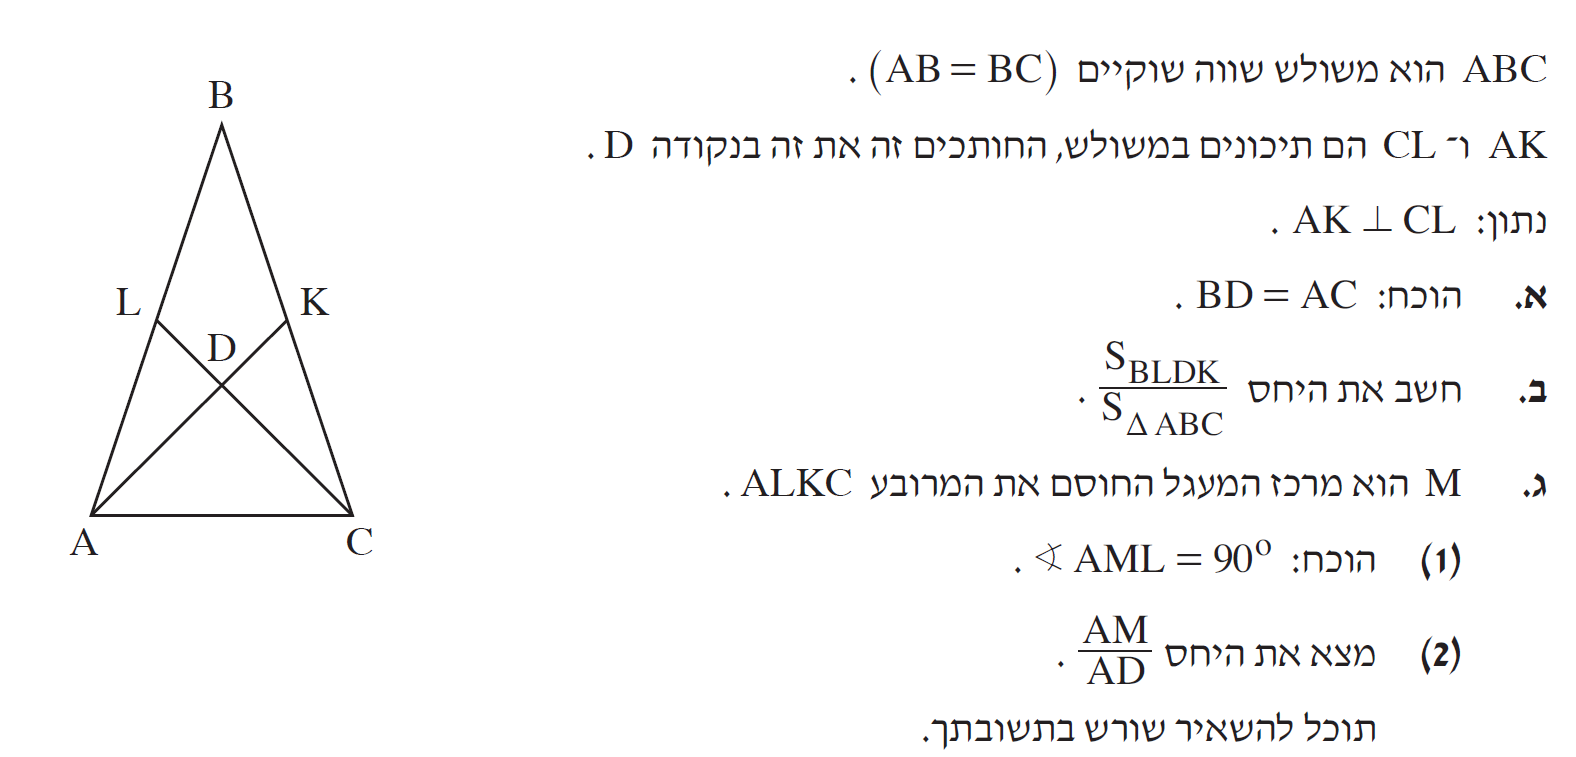
\includegraphics[width=\textwidth]{summer-2018b-4}
\end{center}

\vspace{-3ex}

\textbf{סעיף א}

כאשר יש תיכונים נחתכים מיד חושבים על משפט
$45$
"שלושת התיכונים במשולש נחתכים בנקודה אחת", ובמשפט
$46$
"נקודת חיתוך התיכונים מחלקת כל תיכון ביחס
$2:1$".
$BE$
הוא התיכון מ-%
$B$
ל-%
$AC$,
שחותך את מפגש התיכונים האחרים ב-%
$D$.
$BE\perp AC$
לפי משפט
$6$
"במשולש שווה שוקיים , חוצה זווית הראש, התיכון לבסיס והגובה לבסיס מתלכדים". מכאן קל להראות שהתיכונים
$AK,CL$
שווים.
\begin{center}
\selectlanguage{english}
\begin{tikzpicture}[scale=.7]
\draw[thick] (0,0) coordinate (A) -- (6,0) coordinate (C);
\draw[thick] (A) -- (3,8) coordinate (B) -- (C);
\coordinate (K) at ($(B) ! .5 ! (C)$);
\coordinate (L) at ($(A) ! .5 ! (B)$);
\draw[thick,name path=ak] (A) -- (K);
\draw[thick,name path=cl] (C) -- (L);
\path[name intersections={of=ak and cl,by={D}}];
\fill (A) node[below] {$A$} circle(1.5pt);
\fill (B) node[above] {$B$} circle(1.5pt);
\fill (C) node[below] {$C$} circle(1.5pt);
\fill (D) node[above right,xshift=-2pt,yshift=8pt] {$D$} circle(1.5pt);
\fill (K) node[right] {$K$} circle(1.5pt);
\fill (L) node[left] {$L$} circle(1.5pt);
\draw[rotate=-45] (D) rectangle +(7pt,7pt);
\draw[dashed,thick] (B) |- (A);
\coordinate (E) at ($(A)!.5!(C)$);
\fill (E) node[below] {$E$} circle(1.5pt);
\draw (E) rectangle +(7pt,7pt);
\path (A) -- node[right,yshift=-4pt] {$2a$} (D) -- node[right,yshift=-4pt] {$a$} (K);
\path (C) -- node[left,yshift=-4pt] {$2a$} (D) -- node[left,yshift=-4pt] {$a$} (L);
\path (B) -- node[left] {$2b$} (D) -- node[left] {$b$} (E);
\path (A) -- node[below] {$b?$} (E);
\path (E) -- node[below] {$b?$} (C);
\end{tikzpicture}
\end{center}
אם נוכיח ש-%
$AE=EC=DE$,
נוכיח ש-% 
$BD=2b=2DE=AE+ED=AC$.
לפי משפט
$6$,
$BE$
הוא חוצה זווית של
$\angle ABC$,
וגם של
$\angle ADC$
כי חוצה הזווית והתיכון מתלכדים. נתון ש-%
$AK\perp CL$
כך ש-%
$\angle ADC=90^\circ$,
ולכן 
$\angle ADE,\angle CDE$
שוות ל-%
$\frac{1}{2}\cdot 90^\circ=45^\circ$.
במשולשים ישר זווית
$\triangle ADE,\triangle CDE$,
זוויות חדות של
$45^\circ$,
ולכן גם הזוויות
$\angle DAE,\angle DCE$
שוות
$45^\circ$,
והמשולשים שווה שוקיים. מכאן ש-%
$AE=EC=DE=b$.

אפשרות אחרת, פשוטה יותר, להוכיח
$AE=EC=DE=b$
היא להשתמש במשפט
$86$
"במשולש ישר זווית התיכון ליתר שווה למחצית היתר".


\textbf{סעיף ב}

כדאי לחשב 
$S_{BLDK}$
על ידי חיסור שטח המצולע
$ALDKC$
מהשטח של
$\triangle ABC$,
כי המצולע מורכב ממשולשים ישר זווית וחישוב השטח שלהם קל מאוד:
\erh{12pt}
\begin{equationarray*}{rcl}
S_{ALDKC}&=&2S_{ADL}+S_{ADC}\\
&=&2\cdot \frac{1}{2} AD\cdot DL + \frac{1}{2} AC\cdot DE\\
&=&2a\cdot a + \frac{1}{2}\cdot 2b \cdot b\\
&=&2a^2+b^2\,.
\end{equationarray*}
אפשר להניח שהיחס המבוקש אינו תלוי באורכם של הצלעות, לכן נחפש דרך להביע את שטח המצולע
$S_{ALDKC}$
כפונקציה של
$b$
בלבד. ממשפט פיתגורס על
$\triangle ADE$:
\erh{12pt}
\begin{equationarray*}{rcl}
b^2+b^2&=&(2a)^2=4a^2\\
%b^2&=&2a^2\\
S_{ALDKC}&=&2a^2+b^2=2\cdot\frac{1}{4}(b^2+b^2)+ b^2=2b^2\\
S_{ABC}&=&\frac{1}{2}AC\cdot BE= \frac{1}{2}2b\cdot 3b=3b^2\\
S_{BLDK}&=&S_{ABC}-S_{ALDKC}=3b^2-2b^2=b^2\\
\frac{S_{BLDK}}{S_{ABC}}&=&\frac{b^2}{3b^2}=\frac{1}{3}\,.
\end{equationarray*}

\textbf{סעיף ג}
$(1)$

לא התקדמתי בפתרון עד שציירתי תרשים חדש עם המעגל וראיתי שהזווית ההיקפית
$\angle LKA$
נשענת על המיתר עליו נשענת הזווית המרכזית
$\angle AML$,
כך ש-%
$\angle AML=2\angle LKA$
לפי משפט
$69$
"במעגל, זווית היקפית שווה למחצית הזווית המרכזית הנשענת על אותה הקשת". אבל לפי משפט
$14$
"קטע אמצעים במשולש מקביל לצלע השלישית ושווה למחציתה",
$LK\|AC$.
$\angle KAC=\angle LKA=\alpha$
לפי זוויות מתחלפות, והוכחנו בסעיף הקודם ש-%
$\alpha = 45^\circ$,
לכן,
$\angle AML = 2\alpha=90^\circ$.

\vspace{-1mm}
\begin{center}
\selectlanguage{english}
\begin{tikzpicture}
\clip (-1,-2.2) rectangle +(8,7);
\draw[thick] (0,0) coordinate (A) -- (6,0) coordinate (C);
\path (A) -- (3,8) coordinate (B) -- (C);
\coordinate (K) at ($(B) ! .5 ! (C)$);
\coordinate (L) at ($(A) ! .5 ! (B)$);
\path[name path=ak] (A) -- (K);
\draw[thick,name path=cl] (C) -- (L);
\path[name intersections={of=ak and cl,by={D}}];
\fill (A) node[below,xshift=-4pt] {$A$} circle(1.5pt);
\fill (C) node[below,xshift=4pt] {$C$} circle(1.5pt);
\fill (D) node[above] {$D$} circle(1.5pt);
\fill (K) node[right,xshift=4pt] {$K$} circle(1.5pt);
\fill (L) node[left,xshift=-4pt] {$L$} circle(1.5pt);
\draw[rotate=135] (D) rectangle +(7pt,7pt);
\tkzCircumCenter(A,L,K)\tkzGetPoint{M}
\tkzDrawCircle[thick,name path=circle](M,A)
\fill (M) node[above right] {$M$} circle(1.5pt);
\draw[rotate=110] (M) rectangle +(7pt,7pt);
\draw[thick] (A) -- (M);
\draw[thick,name path=ml] (M) -- (L);
\path[name intersections={of=ak and ml,by={G}}];
\fill (G) node[left,xshift=-4pt] {$G$} circle(1.5pt);
\draw[thick] (A) -- (L) -- (K) -- (C);
\draw[thick] (A) -- (K);
\node[below left,xshift=-8pt] at (K) {$\alpha$};
\node[left,xshift=-6pt,yshift=4pt] at (M) {$2\alpha$};
\draw[thick] ($(A)+(10mm,0)$) arc[start angle=0,end angle=45,radius=9mm];
\node[above right,yshift=10pt,xshift=22pt] at (A) {$\alpha$};
\path (L) -- node[right] {$a$} (D);
\path (A) -- node[left,xshift=4pt,yshift=8pt] {$2a$} (D);
\end{tikzpicture}
\end{center}

\textbf{סעיף ג}
$(2)$

תחילה שמתי לב ש-%
$\triangle MGA\sim \triangle DGL$
כי במשלושים ישר זווית, הזוויות
$\angle MGA=\angle DGL$
קודקודיות. גישה זו לא הצליחה כי לא מצאתי דרך לבטא את הקשר בין
$AD$
לבין 
$AG, GD$.
לבסוף שמתי לב שלמשולשים
$\triangle LDA,\triangle LMA$
יתר משותף, והמשולש
$\triangle LMA$
שווה שוקיים כי שני הצלעות
$AM,ML$
הם רדיוסים. ממשפט פיתגורס:
\erh{12pt}
\begin{equationarray*}{rcl}
AM^2+ML^2&=&AL^2\\
%AM&=&ML\\
2AM^2&=&AL^2\\
LD^2+AD^2&=&AL^2\\
%LD^2&=&a^2\\
a^2+AD^2&=&2AM^2\\
%AD^2&=&4a^2\\
\frac{1}{4}AD^2+AD^2&=&2AM^2\\
\frac{AM}{AD}&=&\sqrt{\frac{5}{8}}\,.
\end{equationarray*}

%%%%%%%%%%%%%%%%%%%%%%%%%%%%%%%%%%%%%%%%%%%%%%%%%%%%%%%%%%%%%%%%%%%

\np

\section{קיץ תשע"ח מועד א}

\begin{center}
\selectlanguage{english}
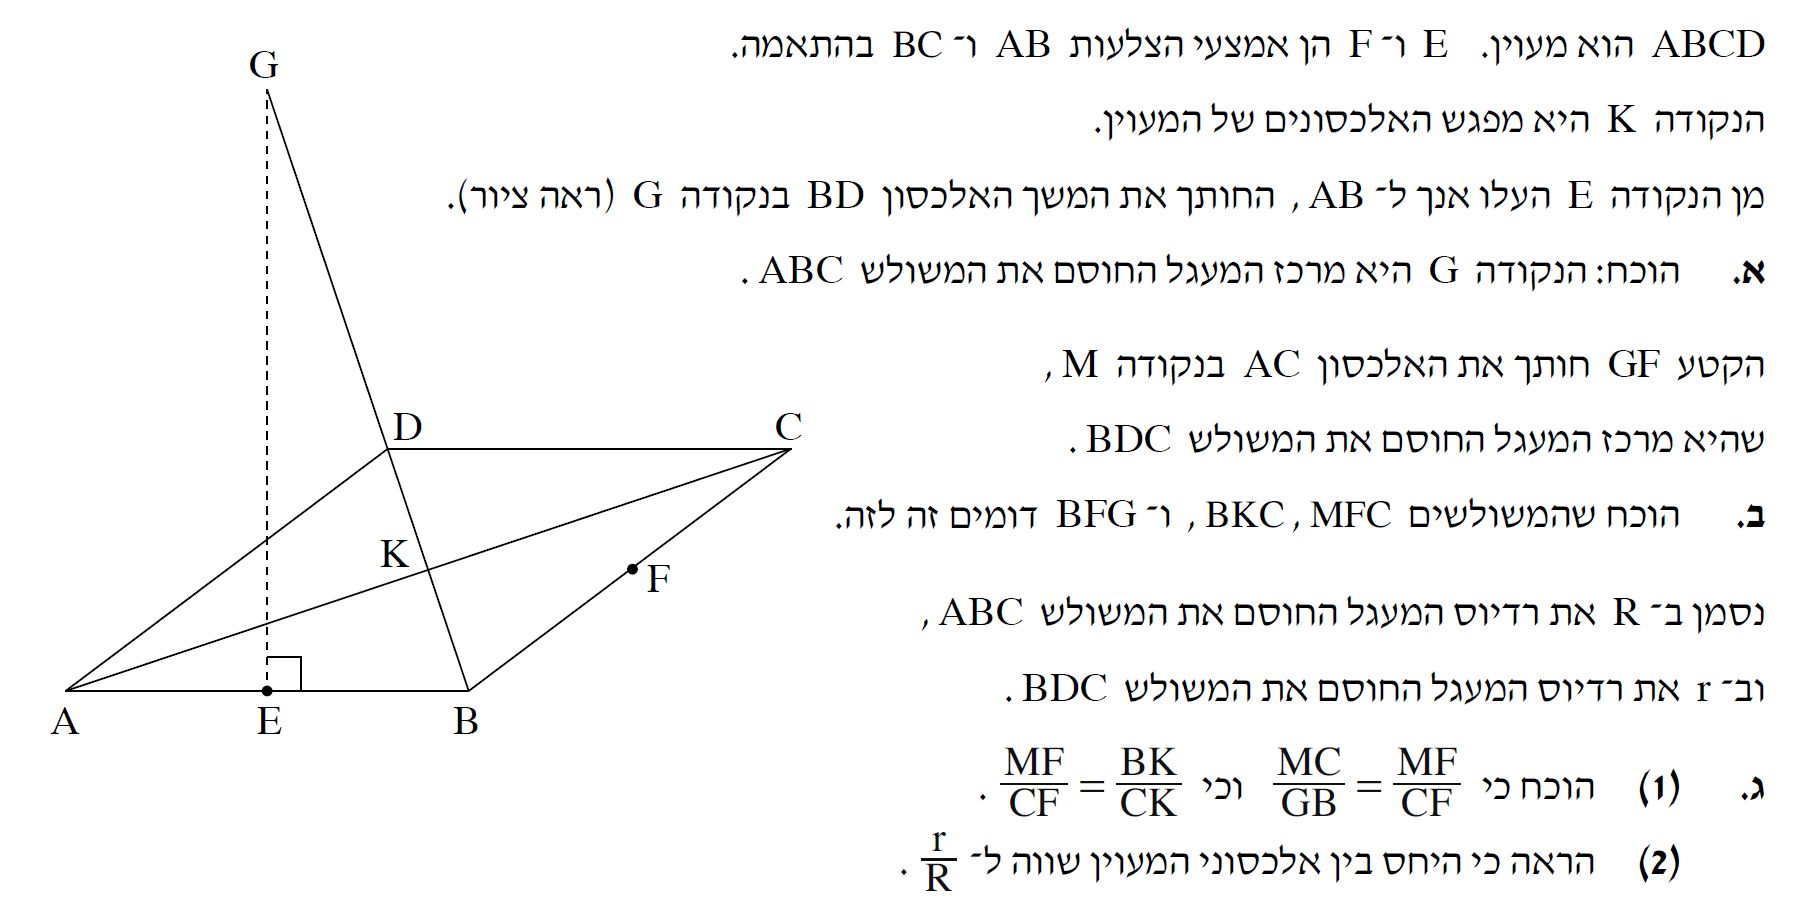
\includegraphics[width=\textwidth]{summer-2018a-4}
\end{center}

\vspace{-2ex}

\textbf{סעיף א}

כדי להוכיח שהנקודה
$G$
היא מרכז של מעגל חוסם נשתמש במשפט
$54$
"במשולש, שלושת האנכים האמצעיים נחתכים בנקודה אחת , שהיא מרכז המעגל החוסם את המשולש". צריך להוכיח ש-%
$GE,GB$
הם אנכים אמצעיים. מעוין הוא מקבילית עם צלעות שווים, וכמקבילית, ניתן להשתמש במשפט 
$28$
"במקבילית האלכסונים חוצים זה את זה". סימנו בציר את אורכי האלכסון
$AC$
ב-%
$b$.
ביחד עם משפט
$35$
"במעוין האלכסונים מאונכים זה לזה", 
$GB$
הוא אנך אמצעי ל-%
$AC$.
נתון שנקודת
$E$
היא אמצע של 
$AB$,
וש-%
$GE$
הוא אנך ל-%
%
$AB$,
ולכן
$G$
היא נקודת החיתוך של שני אנכים אמצעיים ומרכז של מעגל חוסם ל-%
$\triangle ABC$.

\begin{center}
\selectlanguage{english}
\begin{tikzpicture}[scale=.8]
\draw[thick] (0,0) coordinate (A) -- ++(40:5) coordinate (D) -- ++(5,0) coordinate (C);
\draw[thick] (A) -- ++(5,0) coordinate (B) -- (C);
\coordinate (F) at ($(B) ! .5 ! (C)$);
\coordinate (E) at ($(A) ! .5 ! (B)$);
\fill (A) node[below] {$A$} circle(1.5pt);
\fill (B) node[below] {$B$} circle(1.5pt);
\fill (C) node[above] {$C$} circle(1.5pt);
\fill (D) node[above right] {$D$} circle(1.5pt);
\fill (E) node[below] {$E$} circle(1.5pt);
\fill (F) node[right,xshift=2pt] {$F$} circle(1.5pt);
\draw[thick,name path=ac] (A) -- (C);
\path[name path=bg] (B) -- ($(B) ! 2.3 ! (D)$);
\path[name path=ge] (E) -- +(0,7.3);
\path[name intersections={of=ge and bg,by={G}}];
\fill (G) node[above] {$G$} circle(1.5pt);
\draw[dashed,thick] (G) -- (E);
\draw[thick] (G) -- (B);
\path[name intersections={of=ac and bg,by={K}}];
\fill (K) node[above,xshift=5pt,yshift=2pt] {$K$} circle(1.5pt);
\draw[rotate=110] (K) rectangle +(7pt,7pt);
\draw (E) rectangle +(7pt,7pt);
\path (A) -- node[below] {$a$} (E) -- node[below] {$a$} (B);
\path (B) -- node[right,xshift=2pt] {$a$} (F) -- node[right,xshift=2pt] {$a$} (C);
\path (A) -- node[below,near end] {$b$} (K) -- node[below,near start] {$b$} (C);
\end{tikzpicture}
\end{center}

\np

\textbf{סעיף ב}

ההוכחה שהמשולשים דומים תהיה קל יותר אם נצייר מחדש את התרשים תוך הדגשת צלעות המשולשים. לפי משפט 
$35$
האלכסון 
$AC$
הוא אנך אמצעי ל-%
$DB$.
נתון שהנקודה
$M$
היא מרכז המעגל החוסם את
$\triangle BDC$,
ולכן הנקודה
$GF$
שחותכת את 
$CK$
ב-%
$M$
היא אנך אמצעי ל-%
$BC$.
הזווית
$\alpha$
משותפת לשני משולשים ישר זווית, כך ש-%
$\triangle BKC\sim \triangle MFC$.
הזווית
$\beta$
משותפת לשני משולשים ישר זווית, כך ש-%
$\triangle BFG\sim \triangle BKC$
ו-%
$\triangle BFG\sim \triangle BKC \sim \triangle MFC$.

\vspace{-2ex}

\begin{center}
\selectlanguage{english}
\begin{tikzpicture}[scale=.8]
\draw[thick] (0,0) coordinate (A) -- ++(40:5) coordinate (D) -- ++(5,0) coordinate (C);
\draw[thick] (A) -- ++(5,0) coordinate (B) -- (C);
\coordinate (F) at ($(B) ! .5 ! (C)$);
\coordinate (E) at ($(A) ! .5 ! (B)$);
\fill (A) node[below] {$A$} circle(1.5pt);
\fill (B) node[below] {$B$} node[above,xshift=3pt,yshift=4pt] {$\beta$}  circle(1.5pt);
\fill (C) node[above] {$C$} node[below left,xshift=-20pt,yshift=-10pt] {$\alpha$} circle(1.5pt);
\fill (D) node[above right] {$D$} circle(1.5pt);
\fill (E) node[below] {$E$} circle(1.5pt);
\fill (F) node[right] {$F$} circle(1.5pt);
\draw[thick,name path=ac] (A) -- (C);
\path[name path=bg] (B) -- ($(B) ! 2.3 ! (D)$);
\path[name path=ge] (E) -- +(0,7.3);
\path[name intersections={of=ge and bg,by={G}}];
\fill (G) node[above] {$G$} circle(1.5pt);
\draw[thick] (G) -- (B);
\path[name intersections={of=ac and bg,by={K}}];
\fill (K) node[above,xshift=5pt,yshift=2pt] {$K$} circle(1.5pt);
\draw[rotate=110] (K) rectangle +(7pt,7pt);
\draw[thick,dashed,name path=gf] (G) -- (F);
\path[name intersections={of=gf and ac,by={M}}];
\fill (M) node[below,xshift=-4pt,yshift=-4pt] {$M$} circle(1.5pt);
\draw[rotate=130] (F) rectangle +(7pt,7pt);
\draw[ultra thick] (M) -- (F) -- (C) -- cycle;
\draw[ultra thick] (B) -- (K) -- (C) -- cycle;
\draw[ultra thick] (B) -- (F) -- (G) -- cycle;
\path (B) -- node[right,xshift=4pt] {$a$} (F) -- node[right,xshift=-6pt,yshift=-10pt] {$a$} (C);
\end{tikzpicture}
\end{center}

\vspace{-2ex}

\textbf{סעיף ג}
$(1)$

היחס: 
\[
\frac{MC}{GB}=\frac{MF}{BF}=\frac{MF}{CF}
\]
מתקבל מדמיון המשולשים
$\triangle BFG\sim \triangle MFC$
ו-%
$BF=CF$
כי 
$F$
הוא אמצע הצלע
$BC$.

מדמיון המשולשים
$\triangle BKC \sim \triangle MFC$.
מתקבל:
\erh{12pt}
\begin{equationarray*}{rcl}
\frac{MF}{BK}&=&\frac{CF}{CK}\\
\frac{MF}{CF}&=&\frac{BK}{CK}\,.
\end{equationarray*}

\vspace{-2ex}

\textbf{סעיף ג
$(2)$}

מהנתון שהנקודה 
$M$
היא המכרז של המעגל החוסם את
$BDC$,
אנו מקבלים שהאלכסון
$MC$
שווה ל-%
$r$.
בסעיף א הוכחנו שהנקודה 
$G$
היא מרכז המעגל החוסם את
$ABC$,
ולכן 
$GB$
שווה ל-%
$R$.
נחשב את יחס הרדיוסים תוך שימוש ביחס שחישבנו בסעיף ג
$1$
ומשפט 
$29$
שהאלכסונים של מקבילית )מעוין( חוצים אחד את השני:
\[
\frac{r}{R}=\frac{MC}{GB}=\frac{BK}{CK}=\frac{DB/2}{AC/2}=\frac{DB}{AC}\,
\]


%%%%%%%%%%%%%%%%%%%%%%%%%%%%%%%%%%%%%%%%%%%%%%%%%%%%%%%%%%%%%%%%%%%
\np

\section{חורף תשע"ח}

\begin{center}
\selectlanguage{english}
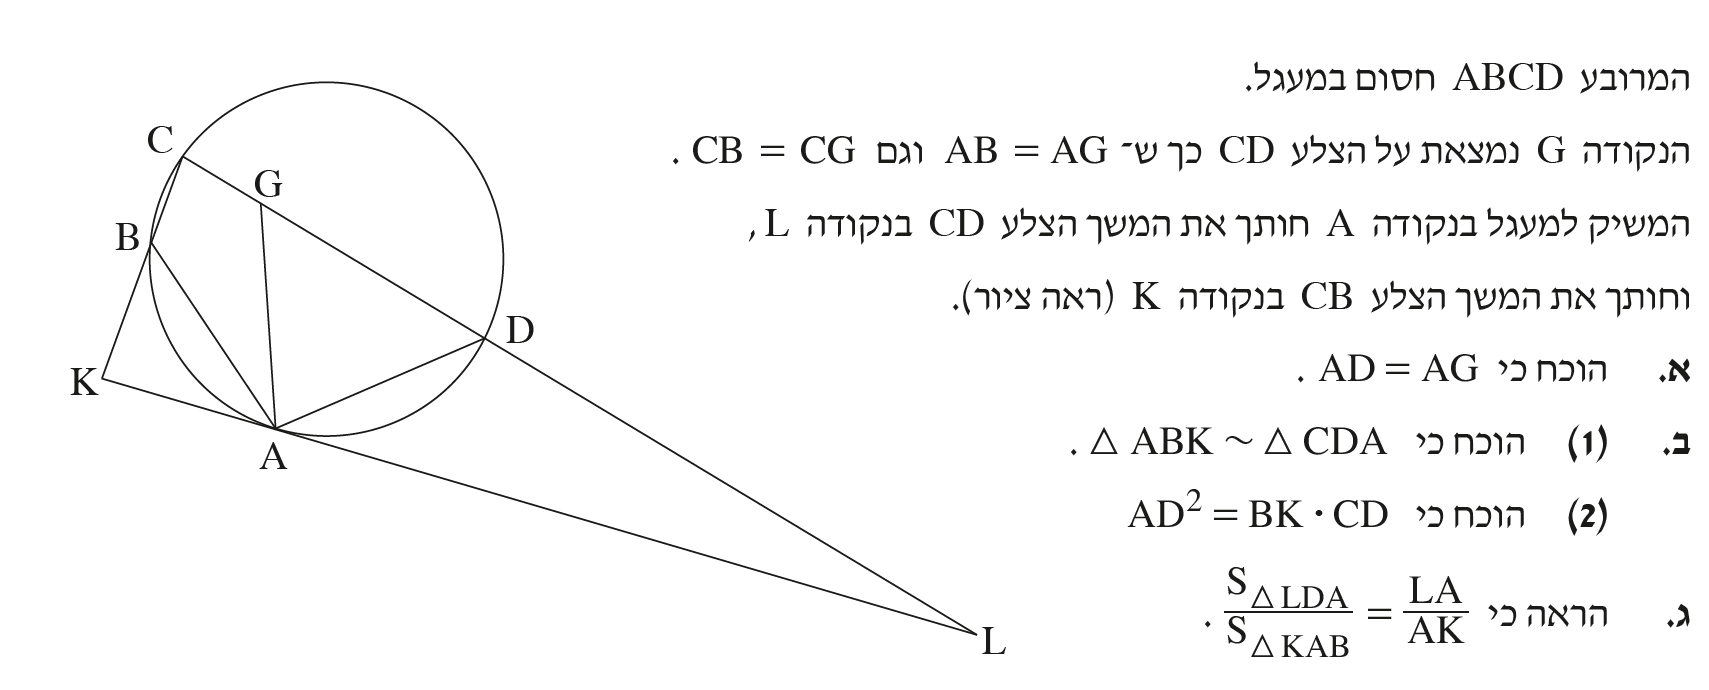
\includegraphics[width=\textwidth]{winter-2018-4}
\end{center}



\textbf{סעיף א}

נתון ש-%
$AB=AG,CB=CG$
כך ש-%
$ABCG$
הוא דלתון, אבל לא ברור בשלב זה אם זה יעזור בפתרון. נתון שהמרובע 
$ABCD$
חסום במעגל, ולפי משפט
$56$
"ניתן לחסום מרובע במעגל אם ורק אם סכום זוג זוויות נגדיות שווה ל-%
$180^\circ$".
סימנו זוויות
$\alpha,\beta$
ו-%
$\alpha'=180-\alpha, \beta'=180-\beta$:
\begin{center}
\selectlanguage{english}
\begin{tikzpicture}[scale=.95]
\coordinate (L) at (60mm,-51mm);
\fill (L) node[right] {$L$} circle(1.5pt);
\node[circle,draw,thick,name path=circle] (O) at (0,0) [minimum size=50mm] {};
\coordinate (A) at (tangent cs:node=O,point={(L)},solution=2);
\fill (A) node[below] {$A$} node[above right,yshift=8pt] {$\alpha'$} circle(1.5pt);
\path[name path=la] (L) -- ($(L)!1.4!(A)$);
\node[circle,name path=abd] (c) at (A) [minimum size=55mm] {};
\path[name intersections={of=circle and abd,by={B,D}}];
\fill (D) node[right,xshift=4pt] {$D$} node[left,xshift=-10pt,yshift=2pt] {$\beta$} circle(1.5pt);
\fill (B) node[left] {$B$} node[below right,xshift=4pt,yshift=5pt] {$\beta'$} circle(1.5pt);
\path[name path=ld] (L) -- ($(L)!2!(D)$);
\path[name intersections={of=circle and ld,by={C}}];
\fill (C) node[above left] {$C$} node[below,xshift=3pt,yshift=-6pt] {$\alpha$} circle(1.5pt);
\draw[thick,name path=lc] (L) -- (C);
\path[name path=cb] (C) -- ($(C)!2.4!(B)$);
\path[name intersections={of=cb and la,by={K}}];
\fill (K) node[below left] {$K$} circle(1.5pt);
\path[name intersections={of=abd and lc,by={dummy,G}}];
\fill (G) node[above] {$G$} circle(1.5pt);
\draw[thick] (A) -- node[left] {$a$} (B);
\draw[thick] (A) -- (D);
\draw[thick] (A) -- node[right] {$a$} (G);
\draw[thick] (L) -- (K);
\draw[thick] (C) -- node[left,xshift=-4pt] {$b$} (B);
\draw[thick] (B) -- (K);
\path (C) -- node[right,near start,xshift=4pt] {$b$} (G);
\draw ($ (A)!.15!(D) $) arc [radius=14pt,start angle=20,delta angle=94];
\draw[dashed] (B) -- (G);
\end{tikzpicture}
\end{center}

אם
$AD=AG$
המשולש
$\triangle GAD$
שווה שוקיים, ולפי הסימונים של הזוויות ננסה להוכיח ש-%
$\angle AGD=\angle ADG=\beta$.
נזכור ש-%
$ABCG$
דלתון והזוויות הצדדיות שלו שוות, כך ש:
\[
\angle AGC=\angle ABC=\beta'\,,\quad\quad \angle AGD=180-(180-\beta)=\beta\,.
\]
\vspace{-10mm}
\begin{quote}
רשימת המשפטים לבגרות לא כוללת משפט על שוויון זוויות בדלתון, אז נצטרך להוכיח אותו. דלתון מוגדר כמרובע עם שני זוגות של צלעות סמוכות שוות, כך שהוא מורכב משני משולשים שווה שוקיים המוצמדים בבסיסיהם )קו מקווקוו בתרשים(:
\[
\angle ABC = \angle ABG + \angle GBC = \angle AGB + \angle BGC = \angle AGC\,.
\]
\end{quote}

\np

\textbf{סעיף ב %
$(1)$}

נדגיש בתרשים את המשולשים
$\triangle ABK,\triangle CDA$
שיש להוכיח שהם דומים. הוספנו לתרשים את הסימון
$\angle ABK=\beta$,
המשלים של 
$\angle ABC=\beta'$.
אם נמצא עוד זוג של זוויות שוות נקבל שהמשולים דומים לפי ז.ז. ננסה להוכיח ש-%
$\angle ACD=\angle BAK$.

$\angle BAK$
היא הזווית בין המשיק
$KA$
והמיתר
$AB$.
לפי משפט
$79$
"זווית בין משיק ומיתר שווה לזווית ההיקפית הנשענת על מיתר זה מצידו השני", 
$\angle BAK=\angle BCA=\gamma$.
לפי משפט
$21$
"האלכסון הראשי בדלתון חוצה את זוויות הראש ...",
$\angle BAK=\angle BCA=\angle ACD=\gamma$.
מכאן ש-%
$\triangle ABK \sim \triangle CDA$
לפי ז.ז.
\begin{center}
\selectlanguage{english}
\begin{tikzpicture}[scale=.95]
\coordinate (L) at (60mm,-51mm);
\node[circle,draw,name path=circle] (O) at (0,0) [minimum size=50mm] {};
\coordinate (A) at (tangent cs:node=O,point={(L)},solution=2);
\fill (A) node[below] {$A$} circle(1.5pt);
\path[name path=la] (L) -- ($(L)!1.4!(A)$);
\node[circle,name path=abd] (c) at (A) [minimum size=55mm] {};
\path[name intersections={of=circle and abd,by={B,D}}];
\fill (D) node[right,xshift=4pt] {$D$} node[left,xshift=-10pt,yshift=2pt] {$\beta$} circle(1.5pt);
\fill (B) node[left] {$B$} node[right,yshift=1pt] {$\beta'$} node[below,xshift=2pt,yshift=-8pt] {$\beta$} circle(1.5pt);
\path[name path=ld] (L) -- ($(L)!2!(D)$);
\path[name intersections={of=circle and ld,by={C}}];
\fill (C) node[above left] {$C$} circle(1.5pt);
\path[name path=lc] (L) -- (C);
\path[name path=cb] (C) -- ($(C)!2.4!(B)$);
\path[name intersections={of=cb and la,by={K}}];
\fill (K) node[below left] {$K$} circle(1.5pt);
\path[name intersections={of=abd and lc,by={dummy,G}}];
\fill (G) node[above] {$G$} circle(1.5pt);
\draw (A) -- (G);
\draw (C) -- (B);
\draw[very thick] (A) -- (B);
\draw[very thick] (A) -- (D);
\draw[very thick] (B) -- (K);
\draw[very thick] (C) -- (A);
\draw[very thick] (A) -- (K);
\draw[very thick] (D) -- (C);
\node at ($(C)+(-8.5mm,-5mm)$) {$\gamma$};
\node at ($(C)+(-6mm,-5.2mm)$) {$?$};
\draw[->] ($(C)+(-4mm,-4mm)$) -- +(13pt,0);
\draw[->] ($(C)+(-4mm,-6mm)$) -- +(22pt,0);
\node at ($(A)+(-8.5mm,-2mm)$) {$\gamma$};
\node at ($(A)+(-6mm,-2.2mm)$) {$?$};
\draw[->] ($(A)+(-7mm,0mm)$) -- +(8pt,12pt);
\end{tikzpicture}
\end{center}

\vspace{-12ex}
דרך אחרת להוכיח ש-%
$\angle BCA=\angle ACD$
היא לשים לב ש-%
$AB=AG=AD$.
נשתמש במשפט
$63$
"במעגל, מיתרים שווים זה לזה אם ורק אם שתי הקשתות המתאימות להם שוות זו לזו" ומשפט
$71$
"במעגל, לקשתות שוות מתאימות זוויות היקפיות שוות", ונקבל
$\angle BCA=\angle ACD$.

\vspace{2ex}
\textbf{סעיף ב %
$(2)$}

לפי 
$\triangle ABK \sim \triangle CDA$
שהוכחנו בהחלק הראשון של הסעיף ולפי
$AB=AD$:
\erh{4pt}
\begin{equationarray*}{rcl}
\frac{AB}{CD}&=&\frac{BK}{AD}\\
AB\cdot AD &=& BK\cdot CD\\
AD^2 &=& BK\cdot CD\,.
\end{equationarray*}

\np

\textbf{סעיף ג}

$LA,AK$
הם הבסיסים של המשולשים
$\triangle LDA, \triangle KAB$
כך שנקבל את היחס המבוקש אם נוכיח שהגבהים שווים. הוכחנו שהיתרים ב-%
$\triangle ADN,\triangle ABM$
שווים
$AB=AD=a$,
כך שנשאר רק להוכיח שהזוויות שוות
$\angle BAK=\angle DAL=\gamma$.
הוכחנו ש-%
$\angle BAK=\angle DCA=\gamma$,
ו-%
$\angle DAL$
היא הזווית בין המשיק
$LA$
והמיתר 
$AD$.
הזווית
$\angle DCA$
נשענת על מיתר זה, כך ש-%
$\angle DCA=\angle DAL$
לפי משפט
$79$,
ו-%
$\angle BAK=\angle DCA=\angle DAL=\gamma$.
כעת ניתן לחשב את השטחים:
\erh{12pt}
\begin{equationarray*}{rcl}
\frac{S_{LDA}}{S_{KAB}}&=&\frac{(LA\cdot DN)/2}{(AK\cdot BM)/2}\\
DN&=&AD\sin \angle DAL=a\sin\gamma\\
BM&=&AB\sin \angle BAK=a\sin\gamma\\
\frac{S_{LDA}}{S_{KAB}}&=&\frac{LA}{AK}\,.
\end{equationarray*}


\begin{center}
\selectlanguage{english}
\begin{tikzpicture}[scale=.95]
\coordinate (L) at (60mm,-51mm);
\fill (L) node[right] {$L$} circle(1.5pt);
\node[circle,draw,thick,name path=circle] (O) at (0,0) [minimum size=50mm] {};
\coordinate (A) at (tangent cs:node=O,point={(L)},solution=2);
\fill (A) node[below] {$A$} circle(1.5pt);
\path[name path=la] (L) -- ($(L)!1.4!(A)$);
\node[circle,name path=abd] (c) at (A) [minimum size=55mm] {};
\path[name intersections={of=circle and abd,by={B,D}}];
\fill (D) node[right,xshift=4pt] {$D$} circle(1.5pt);
\fill (B) node[left] {$B$} circle(1.5pt);
\path[name path=ld] (L) -- ($(L)!2!(D)$);
\path[name intersections={of=circle and ld,by={C}}];
\fill (C) node[above left] {$C$} circle(1.5pt);
\draw[thick,name path=lc] (L) -- (C);
\path[name path=cb] (C) -- ($(C)!2.4!(B)$);
\path[name intersections={of=cb and la,by={K}}];
\fill (K) node[below,yshift=-2pt] {$K$} circle(1.5pt);
\path[name intersections={of=abd and lc,by={dummy,G}}];
\draw[thick] (A) -- node[right,near end] {$a$} (B);
\draw[thick] (A) -- node[above] {$a$} (D);
\draw[thick] (L) -- ($(L)!1.1!(K)$);
\draw[thick] (B) -- (K);
\draw[thick] (A) -- (C);
\draw[thick,dashed] (D) -- ($(A)!(D)!(L)$) coordinate (N);
\draw[thick,dashed] (B) -- ($(A)!(B)!(L)$) coordinate (M);
\fill (N) node[below] {$N$} circle(1.5pt);
\fill (M) node[below left] {$M$} circle(1.5pt);
\draw[rotate=-22] (N) rectangle +(7pt,7pt);
\draw[rotate=70] (M) rectangle +(7pt,7pt);
\node at ($(C)+(-8.5mm,-5mm)$) {$\gamma$};
\draw[->] ($(C)+(-4mm,-4mm)$) -- +(22pt,0);
\node at ($(A)+(-8.5mm,-2mm)$) {$\gamma$};
\draw[->] ($(A)+(-7mm,0mm)$) -- +(8pt,12pt);
\node at ($(A)+(6mm,-8mm)$) {$\gamma$};
\node at ($(A)+(9mm,-8mm)$) {$?$};
\draw[->] ($(A)+(6.1mm,-5.8mm)$) -- +(12pt,18pt);
\end{tikzpicture}
\end{center}


%%%%%%%%%%%%%%%%%%%%%%%%%%%%%%%%%%%%%%%%%%%%%%%%%%%%%%%%%%%%%%%%%%%


\np

\section{קיץ תשע"ז מועד ב}

\begin{center}
\selectlanguage{english}
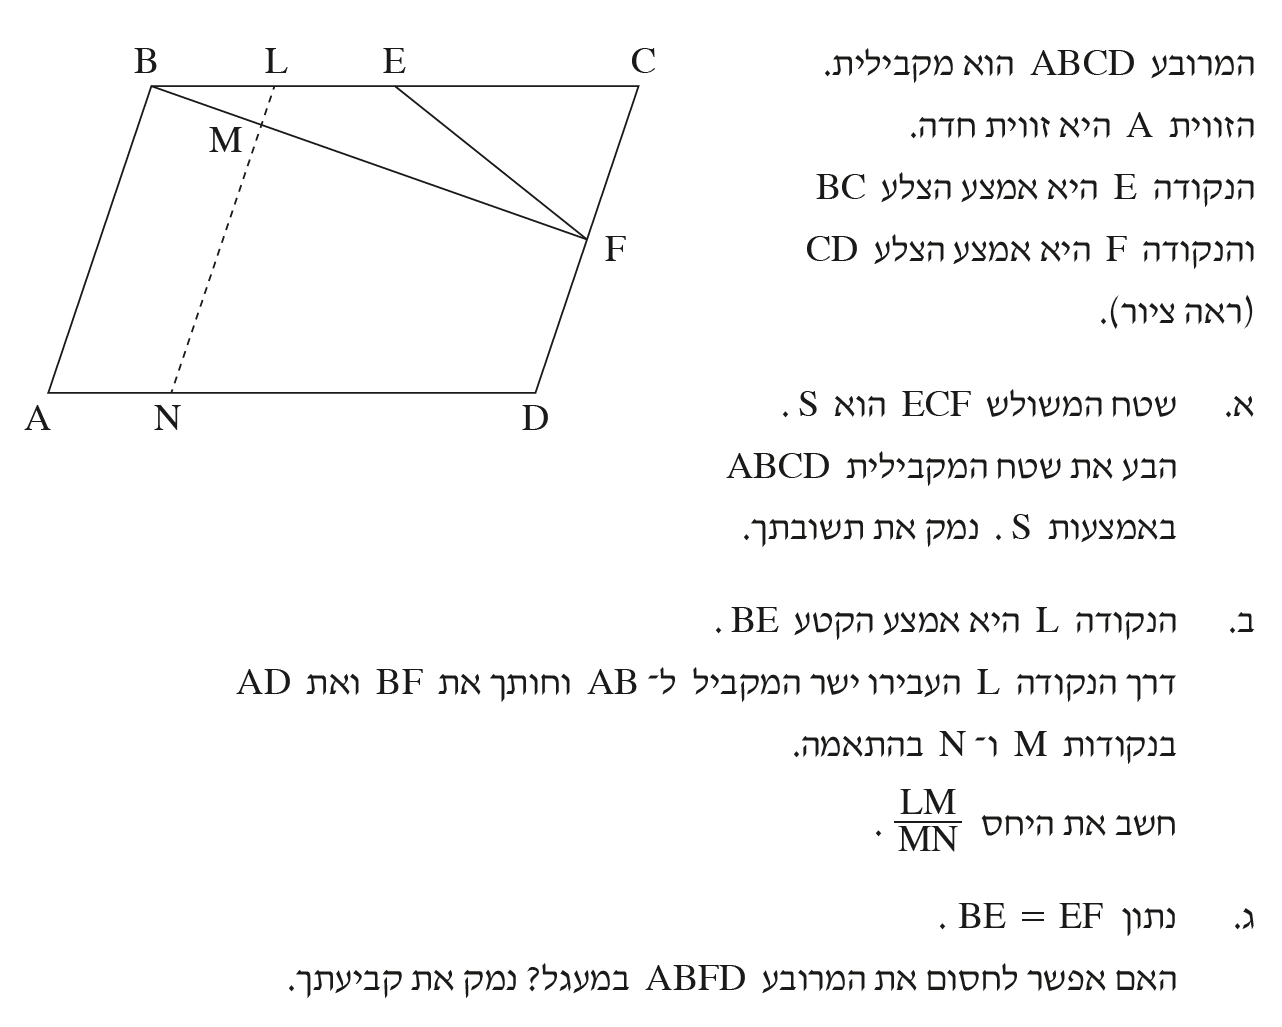
\includegraphics[width=\textwidth]{summer-2017b-4}
\end{center}

\vspace{-2ex}

\textbf{סעיף א}

כדי לחשב את שטח המקבילית באמצעות שטח של משולש נפרק את המקבילית למשולשים. יהי 
$GF$
מקביל ל-%
$BC$
ו-%
$EH$
מקביל ל-%
$CD$.
לפי זוויות מתאימות ומשלימות, המרובעים 
$BEHG,ECFH$
הם מקביליות. בגלל ש-%
$E$
היא נקודת האמצע של
$BC$,
$H$
הוא נקודת האמצע של
$GF=BC$.
מכאן שהמשולשים 
$\triangle ECF,\triangle EHF$
חופפים, ו-%
$S_{EHF}=S_{ECF}=S$.
באותה דרך נוכיח ש-%
$S_{BEH}=S_{BGH}=S$,
ולכן
$S_{BCFG}=4S$.
$GF$
הוא קו אמצעים ומחלק את המקבילית לשני חלקים ששטחם שווה, כך ש-%
$S_{ABCD}=S_{BCFG}+S_{GFDA}=8S$.

\begin{center}
\selectlanguage{english}
\begin{tikzpicture}[scale=.8]
\coordinate (B) at (0,0);
\coordinate (E) at (4,0);
\coordinate (C) at (8,0);
\draw[thick] (B) -- (C);
\draw[thick] (E) -- +(-30:4) coordinate (F);
\draw[thick] (C) -- ($(C) ! 2 ! (F)$) coordinate (D);
\draw[thick] (D) -- +(-8,0) coordinate (A) -- (B);
\fill (A) node[below left] {$A$} circle(1.5pt);
\fill (B) node[above left] {$B$} circle(1.5pt);
\fill (C) node[above right] {$C$} circle(1.5pt);
\fill (D) node[below right] {$D$} circle(1.5pt);
\fill (E) node[above] {$E$} circle(1.5pt);
\fill (F) node[right] {$F$} circle(1.5pt);
\coordinate (G) at ($(A)!.5!(B)$);
\fill (G) node[left] {$G$} circle(1.5pt);
\draw[thick,dashed] (G) -- (F);
\coordinate (H) at ($(G)!.5!(F)$);
\fill (H) node[below] {$H$} circle(1.5pt);
\draw[thick,dashed] (E) -- (H) -- (B);
\end{tikzpicture}
\end{center}

\np

הוכחה אחרת משתמשת במשפט
$5$%
א "שטח מקבילית שווה למכפלת צלע המקבילית בגובה לצלע זו". הגובה של המקבילית באורך כפול מהגובה של המשולש לפי דמיון המשולשים 
$\triangle FCK, \triangle DCJ$:

\vspace{-4ex}

\erh{10pt}
\begin{equationarray*}{rcl}
S_{ECF}&=&\frac{1}{2}ah=S\\
S_{ABCD}&=&2a\cdot 2h=4ah=8S\,.
\end{equationarray*}

\vspace{-4ex}

\begin{center}
\selectlanguage{english}
\begin{tikzpicture}[scale=.8]
\coordinate (B) at (0,0);
\coordinate (E) at (4,0);
\coordinate (C) at (8,0);
\draw[thick] (B) -- (C);
\draw[thick] (E) -- +(-30:4) coordinate (F);
\draw[thick] (C) -- ($(C) ! 2 ! (F)$) coordinate (D);
\draw[thick] (D) -- +(-8,0) coordinate (A) -- (B);
\fill (A) node[below left] {$A$} circle(1.5pt);
\fill (B) node[above left] {$B$} circle(1.5pt);
\fill (C) node[above right] {$C$} circle(1.5pt);
\fill (D) node[below right] {$D$} circle(1.5pt);
\fill (E) node[above] {$E$} circle(1.5pt);
\fill (F) node[below left] {$F$} circle(1.5pt);
\draw[thick,dashed,name path=dj] (D) -- +(2.5,0);
\draw[thick,dashed,name path=cj] (C) -- ($(A)!(C)!(D)$);
\path[name intersections={of=dj and cj,by={J}}];
\fill (J) node[below] {$J$} circle(1.5pt);
\draw (J) rectangle +(7pt,7pt);
\coordinate (K) at ($(C)!.5!(J)$);
\fill (K) node[right] {$K$} circle(1.5pt);
\path (E) -- node[above] {$a$} (C);
\path (A) -- node[below] {$2a$} (D);
\draw[thick,dashed] (F) -- (K);
\draw[<->] ($(C)+(.9,0)$) -- node[fill=white] {$h$} ($(K)+(.9,0)$);
\draw[<->] ($(C)+(1.4,0)$) -- node[fill=white] {$2h$} ($(J)+(1.4,0)$);
\end{tikzpicture}
\end{center}

\vspace{-1ex}

\textbf{סעיף ב}

נקבל יחס בין קטעי קו אם נמצא משולשים דומים שקטעי הקו הם צלעות שלהם. בתרשים להלן הדגשתי משולשים שיכולים להתאים. קטע האמצעים במקבילית מקביל לבסיסים
$BC\|GF$,
ומזוויות מתחלפות
$\angle LBM=\angle MFK$
וזוויות קודקודיות
$\angle LMB=\angle KMF$,
מתקבל:
\[
\triangle LMB \sim \triangle KMF\,.
\]
בתרשים רשמנו את אורכי הקטעים תוך שימוש בנעלמים
$a,b,c$.

\begin{center}
\selectlanguage{english}
\begin{tikzpicture}[scale=.8]
\coordinate (B) at (0,0);
\coordinate (E) at (4,0);
\coordinate (C) at (8,0);
\draw[thick] (B) -- (C);
\path (E) -- +(-30:4) coordinate (F);
\draw[thick] (C) -- ($(C) ! 2 ! (F)$) coordinate (D);
\draw[thick] (D) -- +(-8,0) coordinate (A) -- (B);
\draw[thick,name path=bf] (B) -- (F);
\fill (A) node[below left] {$A$} circle(1.5pt);
\fill (B) node[above left] {$B$} circle(1.5pt);
\fill (C) node[above right] {$C$} circle(1.5pt);
\fill (D) node[below right] {$D$} circle(1.5pt);
%\fill (E) node[above] {$E$} circle(1.5pt);
\fill (F) node[right] {$F$} circle(1.5pt);
\coordinate (G) at ($(A)!.5!(B)$);
\fill (G) node[left] {$G$} circle(1.5pt);
\draw[thick,dashed,name path=gf] (G) -- (F);
\coordinate (L) at (2,0);
\draw[thick,dashed,name path=ln] (L) -- ($(A)!.25!(D)$) coordinate (N);
\fill (L) node[above] {$L$} circle(1.5pt);
\fill (N) node[below] {$N$} circle(1.5pt);
\path[name intersections={of=bf and ln,by={M}}];
\fill (M) node[below left] {$M$} circle(1.5pt);
\path[name intersections={of=gf and ln,by={K}}];
\fill (K) node[below left ] {$K$} circle(1.5pt);
\draw[thick] (L) -- (K);
\draw[thick] (K) -- (F);
\draw[ultra thick] (B) -- node[above] {$a$} (L);
\path (B) -- node[left] {$b$} (G);
\path (G) -- node[left] {$b$} (A);
\path (K) -- node[left] {$b$} (N);
\draw[ultra thick] (K) -- node[below] {$3a$} (F);
\draw[ultra thick] (L) -- node[right] {$c$} (M);
\draw[ultra thick] (M) -- node[left] {$b-c$} (K);
\draw[ultra thick] (B) -- (F);
\end{tikzpicture}
\end{center}

\vspace{-4ex}

\erh{10pt}
\begin{equationarray*}{rcl}
\frac{c}{b-c}&=&\frac{a}{3a}=\frac{1}{3}\\
b&=&4c\\
\frac{LM}{MN}&=&\frac{c}{2b-c}\\
&=&\frac{a}{2\cdot 4c-c}\\
&=&\frac{1}{7}\,.
\end{equationarray*}

\np

\textbf{סעיף ג}

כדי לחסום את המרובע
$ABFD$,
לפי משפט 
$56$
"ניתן לחסום מרובע במעגל אם ורק אם סכום זוג זוויות נגדיות שווה ל-%
$180^\circ$.

בתרשים להלן הוספתי את הנתון 
$BE=EF$.
ראיתי פתרון שמשתמש במשפט
$86$
"במשולש ישר זווית התיכון ליתר שווה למחצית היתר" כדי להוכיח ש-%
$\angle BFC=90^\circ$.
הוכחה זו בעייתית כי משפט
$86$
לא מנוסח כ-"אם ורק אם". לא קשה להוכיח את הכיוון ההפוך כי כל הנקודות הנמצאות במרחק שווה מנקודה 
$E$
נמצאות על מעגל שמרכזו 
$E$.

אפשר לפתור את השאלה ללא שימוש במשפט
$86$
תוך שימוש בעובדות ש: )א( המרובע
$ABCD$
הוא מקבילית, )ב( המשולשים 
$\triangle BEF,\triangle CEF$
שווה שוקיים, )ג( זוויות משלימות ב-%
$E$,
נסמן את הזוויות של המשולש שווה שוקיים
$\triangle BEF$
ב-%
$\alpha$.
מכאן ש-%
$\angle BEF=180-2\alpha$
ולפי זוויות משלימות
$\angle CEF=2\alpha$.
גם משולש 
$\triangle CEF$
הוא שווה שוקיים כך ש-%
$\angle ECF=\angle EFC=90-\alpha$.
ניתן לחבר זוויות ולקבל
$\angle BFC=\angle BFD=90$.

לפי משפט
$26$
"במקבילית כל שתי זוויות נגדיות שוות זו לזו" 
$\angle BAD=\angle BCD=90-\alpha$.
כדי לחסום את המרובע
$ABFD$
חייב להתקיים:
\[
\angle BFD + \angle BAD = 90 + (90-\alpha) = 180-\alpha=180\,.
\]
נתון ש-%
$\angle BAD$
היא זווית חדה שהיא פחות מ-%
$90^\circ$:
\erh{0pt}
\begin{equationarray*}{rcl}
90-\alpha&<&90\\
\alpha&>&0\\
180-\alpha&<&180\,,
\end{equationarray*}
שסותר את הדרישה 
$180-\alpha=180$,
לכן אי אפשר לחסום את המרובע במעגל.

\vspace{2ex}

\begin{center}
\selectlanguage{english}
\begin{tikzpicture}[scale=.8]
\coordinate (B) at (0,0);
\coordinate (E) at (4,0);
\coordinate (C) at (8,0);
\draw[thick] (B) -- (C);
\draw[thick] (E) -- +(-30:4) coordinate (F);
\draw[thick] (C) -- ($(C) ! 2 ! (F)$) coordinate (D);
\draw[thick] (D) -- +(-8,0) coordinate (A) -- (B);
\draw[thick,name path=bf] (B) -- (F);
\fill (A) node[below left] {$A$} circle(1.5pt);
\fill (B) node[above left] {$B$} circle(1.5pt);
\fill (C) node[above right] {$C$} circle(1.5pt);
\fill (D) node[below right] {$D$} circle(1.5pt);
\fill (E) node[above] {$E$} circle(1.5pt);
\fill (F) node[right] {$F$} circle(1.5pt);
\path (B) -- node[above] {$a$} (E) -- node[above] {$a$} (C);
\path (E) -- node[above] {$a$} (F);
\draw[rotate=165] (F) rectangle +(7pt,7pt);
\node[below right,xshift=28pt,yshift=2pt] at (B) {$\alpha$};
\node[above left,xshift=-28pt,yshift=8pt] at (F) {$\alpha$};
\node[below left,xshift=0pt,yshift=2pt] at (C) {$90-\alpha$};
\node[above right,xshift=6pt,yshift=2pt] at (A) {$90-\alpha$};
\node[below left,xshift=-10pt,yshift=-2pt] at (F) {$90$};
\node[above,xshift=40pt,yshift=2pt] at (F) {$90-\alpha$};
\node[below left,xshift=4pt,yshift=2pt] at (E) {$180-2\alpha$};
\node[below right,xshift=16pt,yshift=2pt] at (E) {$2\alpha$};
\draw[->] ($(F)+(20pt,10pt)$) -- +(-25pt,0);
\end{tikzpicture}
\end{center}

%%%%%%%%%%%%%%%%%%%%%%%%%%%%%%%%%%%%%%%%%%%%%%%%%%%%%%%%%%%%%%%%%%%

\np

\section{קיץ תשע"ז מועד א}

\begin{center}
\selectlanguage{english}
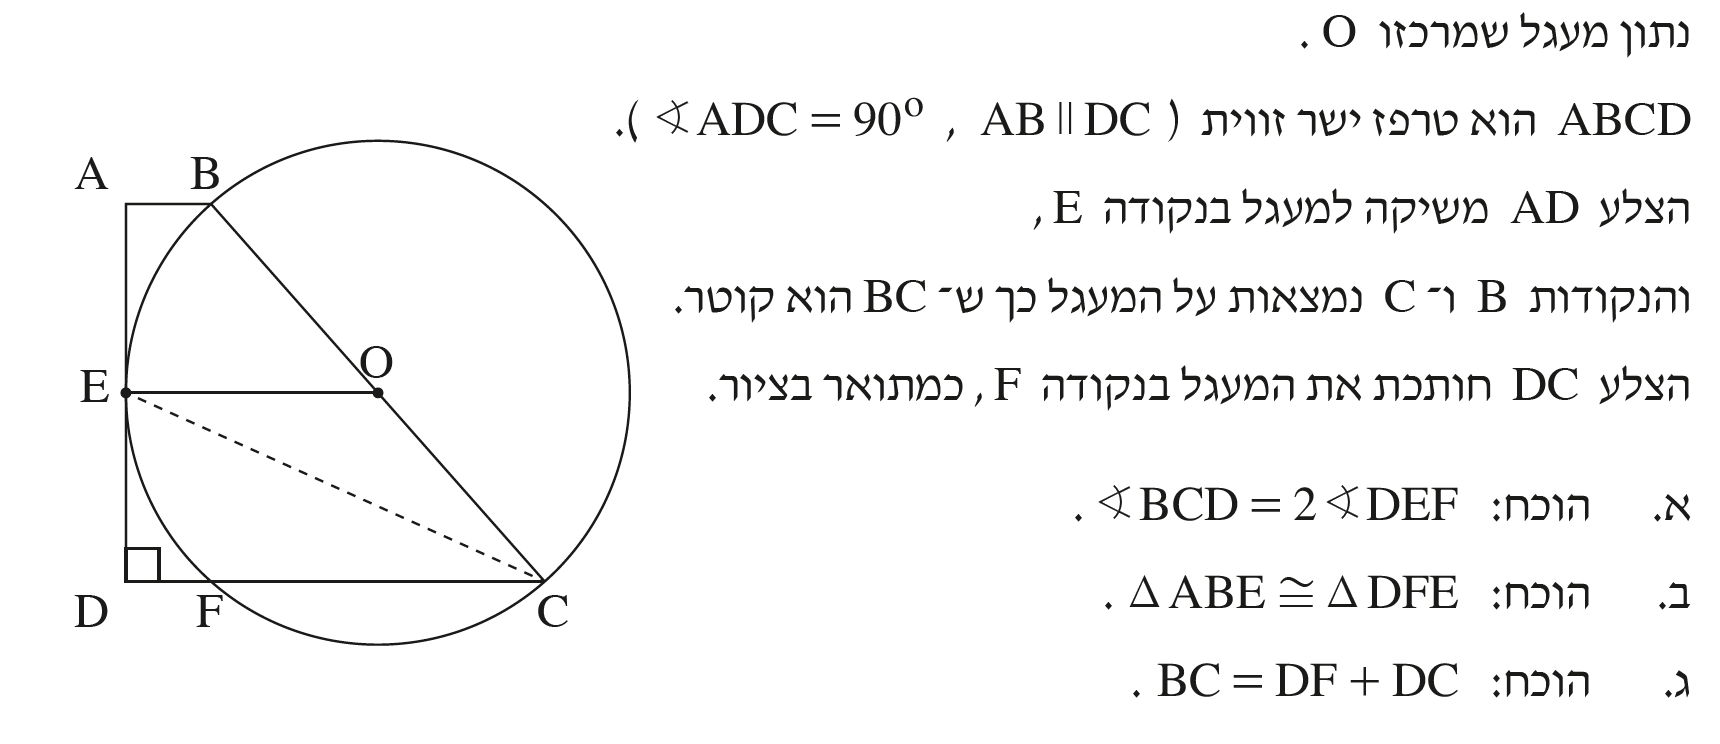
\includegraphics[width=\textwidth]{summer-2017a-4}
\end{center}

\vspace{-3ex}

\textbf{סעיף א}

השאלה שואלת על זוויות ויש לנו קווים מקבילים, משיק, זווית ישרה. ננסה להסיק מסקנות על זזויות. מחברי השאלה סיפקו רמז: הקו 
$EC$.
$\angle DEF$
היא הזווית בין המשיק
$ED$
לבין במיתר 
$EF$
המסומן בתרשים. לפי משפט 
$79$
"זווית בין משיק ומיתר שווה לזווית ההיקפית הנשענת על מיתר זה מצידו השני",
$\angle DEF$
שווה להזווית ההיקפית
$\angle ECF$.
סימנו את שתי הזוויות ב-%
$\alpha$.

נקבל את הערך של
$\angle BCD$
אם נידע את ערכה של
$\angle ECO$.
נתון ש-%
$AB\|DC,\angle ADC=90^\circ$.
המשיק מאונך לרדיוס
$EO$,
ולכן, 
$EO\|DC,EO\perp AD$,
ו-%
$\angle OEC=\alpha=\angle ECB$
לפי זווית מתחלפות. המשולש
$\triangle ECO$
שווה שוקיים ולכן
$\angle ECO=\alpha$,
ו-%
$\angle BCD=2\alpha= 2\angle{DEF}$.

\begin{center}
\selectlanguage{english}
\begin{tikzpicture}[scale=.8]
\coordinate (O) at (0,0);
\fill (O) node[right] {$O$} circle(1.5pt);
\draw[thick,name path=circle] (O) circle(3cm);
\coordinate (E) at (-3,0);
\fill (E) node[left] {$E$} node[below right,xshift=22pt] {$\alpha?$} circle(1.5pt);
\draw[thick] (E) -- +(0,2.5) coordinate (A);
\fill (A) node[above left] {$A$} circle(1.5pt);
\draw[thick] (E) -- +(0,-2.5) coordinate (D);
\fill (D) node[below left] {$D$} circle(1.5pt);
\path[name path=db] (D) -- +(6,0);
\path[name intersections={of=db and circle,by={F,C}}];
\fill (C) node[below right] {$C$} node[above left,xshift=-18pt] {$\alpha$} node[above left,xshift=-16pt,yshift=16pt] {$\alpha?$} circle(1.5pt);
\fill (F) node[below] {$F$} circle(1.5pt);
\path[name path=ab] (A) -- +(2,0);
\path[name intersections={of=ab and circle,by={B}}];
\fill (B) node[above] {$B$} circle(1.5pt);
\draw[thick] (A) -- (B) -- (C) -- (D);
\draw[thick] (E) -- node[above] {$r$} (O) -- node[right] {$r$} (C);
\draw[thick,dashed] (C) -- (E) -- (F);
\node at (-40mm,-5mm) {$\alpha$};
\draw[->] (-39mm,-5mm) -- +(11mm,0);
\draw (E) rectangle +(7pt,7pt);
\draw (D) rectangle +(7pt,7pt);
\draw[rotate=-90] (A) rectangle +(7pt,7pt);
\end{tikzpicture}
\end{center}
הוכחה אחרת משתמשת במשפט
$103$
"אם מנקודה שמחוץ למעגל יוצאים חותך ומשיק, אז מכפלת החותך בחלקו החיצוני שווה לריבוע המשיק". לכן:
\vspace{-3mm}
\erh{10pt}
\begin{equationarray*}{rcl}
ED^2&=&DC\cdot DF\\
\frac{ED}{DF}&=&\frac{DC}{ED}\\
\triangle EDF &\sim& \triangle CDE\,.
\end{equationarray*}

\np

נשתמש במשפט
$69$
"במעגל, זווית היקפית שווה למחצית הזווית המרכזית הנשענת על אותה הקשת", בזוויות המתחלפות 
$\angle BOE=\angle BCD$
ובדמיון המשולשים 
$\triangle EDF \sim \triangle CDE$
שכבר הוכחנו:
\erh{6pt}
\begin{equationarray*}{rcl}
\angle BCD &=& \angle BOE\\
&=& 2\cdot \angle BCE\\
\angle ECD &=& \angle BCD-\angle BCE\\
&=&\angle BCD - \angle BCD/2\\
\angle DEF &=& \angle BCD/2\,.
\end{equationarray*}

\vspace{-4ex}

\textbf{סעיף ב}

שני המשולשים
$\triangle ABE\cong\triangle DFE$
כי הם ישר זווית וצלע באחד המשולשים שווים לזווית וצלע מקבילים במשלוש השני, כי ביחד עם הזווית הישרה יש חפיפה לפי ז.צ.ז. 

נתון ש-%
$BC$
הוא קוטר שמרכזו 
$O$
ולכן
$BO=OC=r$.
נפעיל את השפט
$44$
"בטרפז, ישר החוצה שוק אחת ומקביל לבסיסים, חוצה את השוק השנייה" על הטרפז
$ABCD$,
כדי לקבל
$AE=DE=a$.
נצייר את המיתר
$BE$
ונקווה שהזווית 
$\angle AEB$
בין המיתר ומשיק יהיה שווה לזווית
$\angle DEF=\alpha$
במשלוש השני. לפי משפט
$79$,
$\angle AEB=\angle ECO$,
הזווית ההיקפית.
אבל כבר הוכחנו שזווית זו שווה ל-%
$\angle ECO=\angle DEF=\alpha$.
\begin{center}
\selectlanguage{english}
\begin{tikzpicture}[scale=.8]
\coordinate (O) at (0,0);
\fill (O) node[right] {$O$} node[above left,xshift=-4pt] {$2\alpha$} circle(1.5pt);
\draw[thick,name path=circle] (O) circle(3cm);
\coordinate (E) at (-3,0);
\fill (E) node[left] {$E$} circle(1.5pt);
\draw[thick] (E) -- node[left] {$a$} +(0,2.5) coordinate (A);
\fill (A) node[above left] {$A$} circle(1.5pt);
\draw[thick] (E) -- node[left] {$a$} +(0,-2.5) coordinate (D);
\fill (D) node[below left] {$D$} circle(1.5pt);
\path[name path=db] (D) -- +(6,0);
\path[name intersections={of=db and circle,by={F,C}}];
\fill (C) node[below right] {$C$} node[above left,xshift=-16pt,yshift=14pt] {$\alpha$} node[above left,xshift=-20pt,yshift=2pt] {$\alpha$} circle(1.5pt);
\fill (F) node[below] {$F$} circle(1.5pt);
\path[name path=ab] (A) -- +(2,0);
\path[name intersections={of=ab and circle,by={B}}];
\fill (B) node[above] {$B$} circle(1.5pt);
\draw[thick] (A) -- (B) -- (C) -- (D);
\draw[thick] (E) -- (O) -- node[right] {$r$} (C);
\draw[thick,dashed] (C) -- (E) -- (F);
\draw[thick,dashed] (B) -- (E);
\node at (-43mm,-5mm) {$\alpha$};
\draw[->] (-39mm,-5mm) -- +(11mm,0);
\node at (-43mm,5mm) {$\alpha?$};
\draw[->] (-39mm,5mm) -- +(11mm,0);
\draw (E) rectangle +(7pt,7pt);
\draw (D) rectangle +(7pt,7pt);
\draw[rotate=-90] (A) rectangle +(7pt,7pt);
\path (O) -- node[right] {$r$} (B);
\end{tikzpicture}
\end{center}
הוכחה אחרת מחשבת זוויות מהשולש שווה שוקיים
$\triangle BOE$.
$\angle BOE=2\alpha$
ולכן
$\angle BEO = \angle OBE = 90-\alpha$
ו-%
$\angle AEB=\alpha=\angle DEF$.
ביחד עם 
$AE,ED$,
$\triangle ABE, \triangle DFE$
חופפים.
\np

\textbf{סעיף ג}

האורך של 
$BC$
הוא 
$2r$,
כך שעלינו להוכיח ש-%
$DF+DC=2r$.
אם נפשט את התרשים נראה ש-%
$EO$
הוא קטע אמצעים של הטרפז
$ABCD$,
כי
$BO=OC=r$
ו-%
$AE=ED$
לפי הסעיף הקודם. לפי משפט
$43$
"קטע האמצעים בטרפז מקביל לבסיסים ושווה למחצית סכומם":
\erh{10pt}
\begin{equationarray*}{rcl}
EO&=&\frac{1}{2}(AB+DC)\\
&=&\frac{1}{2}(DF+DC)=r\,,
\end{equationarray*}
כי 
$AB=DF$
לפי משולשים חופפים שהוכחנו בסעיף הקודם, ו-%
$EO$
הוא רדיוס. מכאן ש-%
$BC=2r=DF+DC$.
\begin{center}
\selectlanguage{english}
\begin{tikzpicture}[scale=.8]
\coordinate (O) at (0,0);
\fill (O) node[right] {$O$} circle(1.5pt);
\draw[thick,name path=circle] (O) circle(3cm);
\coordinate (E) at (-3,0);
\fill (E) node[left] {$E$} circle(1.5pt);
\draw[thick] (E) -- +(0,2.5) coordinate (A);
\fill (A) node[above left] {$A$} circle(1.5pt);
\draw[thick] (E) -- +(0,-2.5) coordinate (D);
\fill (D) node[below left] {$D$} circle(1.5pt);
\path[name path=db] (D) -- +(6,0);
\path[name intersections={of=db and circle,by={F,C}}];
\fill (C) node[below right] {$C$} circle(1.5pt);
\fill (F) node[below] {$F$} circle(1.5pt);
\path[name path=ab] (A) -- +(2,0);
\path[name intersections={of=ab and circle,by={B}}];
\fill (B) node[above] {$B$} circle(1.5pt);
\draw[thick] (A) -- (B) -- (C) -- (D);
\draw[thick] (E) -- node[above] {$r$} (O) -- node[right] {$r$} (C);
\draw (E) rectangle +(7pt,7pt);
\draw (D) rectangle +(7pt,7pt);
\draw[rotate=-90] (A) rectangle +(7pt,7pt);
\path (O) -- node[right] {$r$} (B);
\end{tikzpicture}
\end{center}
הוכחה אחרת משתמשת במשפט פיתגורס ומשפט 
$103$
על משיק וקו חותך. נסמן את אורכי הצלעות באיור ונקבל:
\erh{4pt}
\begin{equationarray*}{rcl}
a^2&=&bc\\
BC^2&=& (2a)^2 + (c-b)^2\\
&=&4bc+c^2-2bc+b^2\\
&=&c^2+2bc+b^2\\
&=&(c+b)^2\\
BC&=&c+b=DC+DF\,.
\end{equationarray*}
\vspace{-2mm}
\begin{center}
\selectlanguage{english}
\begin{tikzpicture}[scale=.8]
\coordinate (O) at (0,0);
\fill (O) node[right] {$O$} circle(1.5pt);
\path[thick,name path=circle] (O) circle(3cm);
\coordinate (E) at (-3,0);
\fill (E) node[left] {$E$} circle(1.5pt);
\draw[thick] (E) -- +(0,2.5) coordinate (A);
\fill (A) node[above left] {$A$} circle(1.5pt);
\draw[thick] (E) -- +(0,-2.5) coordinate (D);
\fill (D) node[below left] {$D$} circle(1.5pt);
\path[name path=db] (D) -- +(6,0);
\path[name intersections={of=db and circle,by={F,C}}];
\fill (C) node[below right] {$C$} circle(1.5pt);
\fill (F) node[below] {$F$} circle(1.5pt);
\path[name path=ab] (A) -- +(2,0);
\path[name intersections={of=ab and circle,by={B}}];
\fill (B) node[above] {$B$} circle(1.5pt);
\draw[thick] (A) -- (B) -- (C) -- (D);
\draw[thick] (E) -- (O) -- (C);
\draw (E) rectangle +(7pt,7pt);
\draw (D) rectangle +(7pt,7pt);
\draw (F) rectangle +(7pt,7pt);
\draw[rotate=-90] (A) rectangle +(7pt,7pt);
\draw[thick] (B) -- (F);
\path (E) -- node[left] {$a$} (D);
\path (-1.5,0) -- node[left] {$a$} (F);
\path (D) -- node[below] {$b$} (F);
\draw[<->] (-3,-3.2) -- node[fill=white] {$c$} +(4.67,0);
\end{tikzpicture}
\end{center}

%%%%%%%%%%%%%%%%%%%%%%%%%%%%%%%%%%%%%%%%%%%%%%%%%%%%%%%%%%%%%%%%%%%


\section{חורף תשע"ז}

\begin{center}
\selectlanguage{english}
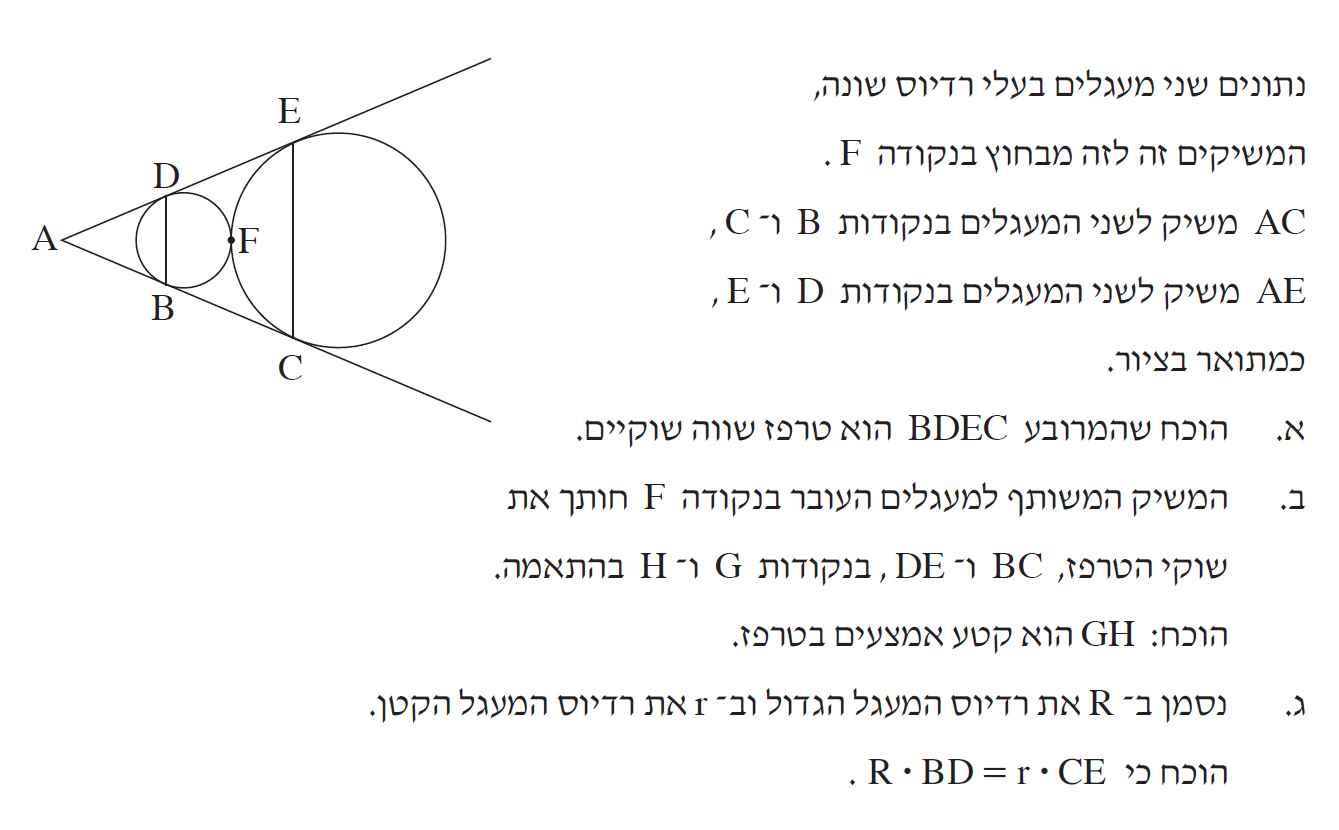
\includegraphics[width=\textwidth]{winter-2017-4}
\end{center}
\vspace{-4ex}
\textbf{סעיף א}

המשפט הרלוונטי ביותר הוא משפט
$80$
"שני משיקים למעגל היוצאים מאותה נקודה שווים זה לזה". נפעיל אותו על
$AC,AE$:
\[
\erh{0pt}
\begin{array}{l}
AD=AB=a\\
AE=AC=a+b\\
DE=BC=b\,.
\end{array}
\]
אם נוכיח ש-%
$DB\|EC$,
המרובע
$BDEC$
יהיה טרפז לפי ההגדרה והוכחנו שהוא שווה שוקיים.

לפי התרשים
$\triangle ADB\sim \triangle AEC$
וזה יכול לתרום לפתרון. המשולשים דומים כי יש להם זווית משותפת ב-%
$A$
והוכחנו ש-%
$\frac{AD}{AE}=\frac{a}{a+b}=\frac{AB}{AC}$,
כך שהמשולשים דומים לפי צ.ז.צ. המשולשים
$\triangle ADB,\triangle AEC$
שווה שוקיים, ולכן לפי משפט
$6$
"במשולש שווה שוקיים , חוצה זווית הראש, התיכון לבסיס והגובה לבסיס מתלכדים". הקו 
$c$,
חוצה הזווית 
$\angle A$,
הוא גם גובה. מכאן שבסיסי המשולשים
$DB, EC$
מאונכים שניהם לקו
$c$
ו-%
$DB\perp EC$.
\begin{center}
\selectlanguage{english}
\begin{tikzpicture}[scale=.7]
\coordinate [label=left:$A$] (A) at (0,0);
\fill (A) circle(1.5pt);
\node[circle,draw,thick] (o1) at (5.4,0) [minimum size=2.7cm] {};
\node[circle,draw,thick] (o2) at (9,0) [minimum size=4.5cm] {};
\coordinate (F) at (6.75,0);
\coordinate (B) at (tangent cs:node=o1,point={(A)},solution=1);
\coordinate (D) at (tangent cs:node=o1,point={(A)},solution=2);
\coordinate (C) at (tangent cs:node=o2,point={(A)},solution=1);
\coordinate (E) at (tangent cs:node=o2,point={(A)},solution=2);
\fill (B) node[below] {$B$} circle(1.5pt);
\fill (D) node[above] {$D$} circle(1.5pt);
\fill (F) node[above right] {$F$} circle(1.5pt);
\fill (C) node[below] {$C$} circle(1.5pt);
\fill (E) node[above] {$E$} circle(1.5pt);
\draw[thick] (A) -- ($(A) !1.2! (E)$);
\draw[thick] (A) -- ($(A) !1.2! (C)$);
\draw[thick,name path=db] (D) -- (B);
\draw[thick,name path=ec] (E) -- (C);
\draw[thick,dashed,name path=dot] (0,0) -- node[above,near end,xshift=15mm] {$c$} (12,0);
\path[name intersections={of=db and dot,by={M}}];
\path[name intersections={of=ec and dot,by={N}}];
\fill (M) circle(1.5pt);
\fill (N) circle(1.5pt);
\draw (M) rectangle +(7pt,7pt);
\draw (N) rectangle +(7pt,7pt);
\path (A) -- node[above] {$a$} (D);
\path (A) -- node[below] {$a$} (B);
\path (D) -- node[above] {$b$} (E);
\path (B) -- node[below] {$b$} (C);
\end{tikzpicture}
\end{center}

\np

\textbf{סעיף ב}

במבט ראשון נראה שכדאי לעבוד עם משפט 
$43$
"קטע האמצעים בטרפז מקביל לבסיסים ושווה למחצית סכומם", כאן, 
$GH=\frac{1}{2}(BD+CE)$.
תחילה עלה בדעתי שאפשר להשתמש בנוסחה לשטח של טרפז שהיא:
\[
S_{BDEC}=h\cdot\frac{1}{2}(BD+CE)\,,
\]
אבל זה לא הוביל לפתרון. אחר כך חשבתי לחפש משולשים כדי להשתמש במשפט
$14$
"קטע אמצעים במשולש מקביל לצלע השלישית ושווה למחציתה", אבל לא מצאתי משולש מתאים.

לאחר פישוט של התרשים שמתי לב ש-%
$H,G$
הן נקודות הניתן להפעיל עליהן את משפט 
$80$
שכבר השתמשתי בסעיף א. 
$DH=HF=x$
ו-%
$HE=HF=y$,
ולכן
$DH=HE$.
אותה הוכחה מראה ש-%
$BG=GC$,
ו-%
$GH$
הוא קטע אמצעים של הטרפז.

\begin{center}
\selectlanguage{english}
\begin{tikzpicture}[scale=.8]
\coordinate [label=left:$A$] (A) at (0,0);
\fill (A) circle(1.5pt);
\node[circle,draw,thick] (o1) at (5.4,0) [minimum size=2.7cm] {};
\node[circle,draw,thick] (o2) at (9,0) [minimum size=4.5cm] {};
\coordinate (F) at (6.75,0);
\path[name path=gh] (6.75,-2.4) -- (6.75,2.4);
\coordinate (B) at (tangent cs:node=o1,point={(A)},solution=1);
\coordinate (D) at (tangent cs:node=o1,point={(A)},solution=2);
\coordinate (C) at (tangent cs:node=o2,point={(A)},solution=1);
\coordinate (E) at (tangent cs:node=o2,point={(A)},solution=2);
\fill (B) node[below] {$B$} circle(1.5pt);
\fill (D) node[above] {$D$} circle(1.5pt);
\fill (F) node[above right] {$F$} circle(1.5pt);
\fill (C) node[below] {$C$} circle(1.5pt);
\fill (E) node[above] {$E$} circle(1.5pt);
\draw[thick,name path=ae] (A) -- ($(A) !1.2! (E)$);
\draw[thick,name path=ac] (A) -- ($(A) !1.2! (C)$);
\draw[thick] (D) -- (B);
\draw[thick] (E) -- (C);
\path[name intersections={of=ac and gh,by={G}}];
\path[name intersections={of=ae and gh,by={H}}];
\fill (G) node[below] {$G$} circle(1.5pt);
\fill (H) node[above] {$H$} circle(1.5pt);
\draw[thick] (G) -- (H);
\path (D) -- node[above] {$x$} (H);
\path (H) -- node[above] {$y$} (E);
\path (H) -- node[right,xshift=20pt] {$x,y$} (F);
\draw[<-] (6.75,9mm) -- +(8mm,0);
\end{tikzpicture}
\end{center}

\textbf{סעיף ג}

ניתן לכתוב את הטענה שיש להוכיח כיחס:
\[
\frac{BD}{CD}=\frac{r}{R}\,.
\]
נוכיח ש-%
$\triangle BO_1D\sim\triangle CO_2E$,
כאשר 
$O_1,O_2$
הן מרכזי המעגלים. המשולשים מורכבים משני משולשים חופפים
$\triangle MO_1D, \triangle MO_1B$
ו-%
$\triangle NO_2E, \triangle NO_2C$,
כך שמספיק להוכיח דימיון של זוג משולשים קטנים. כבר הוכחנו ש-%
$DB\|EC$
והזווית בין רדיוס למשיק היא זוויות ישרה, ולכן:
\[
\angle MDO_1=90-\angle MDA=90-\angle NEA=\angle NEO_2\,.
\]
$\triangle BO_1D\sim\triangle CO_2E$
לפי ז.ז.
\begin{center}
\selectlanguage{english}
\begin{tikzpicture}[scale=.7]
\coordinate [label=left:$A$] (A) at (0,0);
\fill (A) circle(1.5pt);
\coordinate (center1) at (5.4,0);
\coordinate (center2) at (9,0);
\node[circle,draw,thick] (o1) at (center1) [minimum size=2.7cm] {};
\node[circle,draw,thick] (o2) at (center2) [minimum size=4.5cm] {};
\coordinate (F) at (6.75,0);
\path[name path=gh] (6.75,-2.2) -- (6.75,2.2);
\coordinate (B) at (tangent cs:node=o1,point={(A)},solution=1);
\coordinate (D) at (tangent cs:node=o1,point={(A)},solution=2);
\coordinate (C) at (tangent cs:node=o2,point={(A)},solution=1);
\coordinate (E) at (tangent cs:node=o2,point={(A)},solution=2);
\fill (B) node[below] {$B$} circle(1.5pt);
\fill (D) node[above] {$D$} circle(1.5pt);
\fill (C) node[below] {$C$} circle(1.5pt);
\fill (E) node[above] {$E$} circle(1.5pt);
\draw[thick,name path=ae] (A) -- ($(A) !1.2! (E)$);
\draw[thick,name path=ac] (A) -- ($(A) !1.2! (C)$);
\draw[thick,name path=db] (D) -- (B);
\draw[thick,name path=ec] (E) -- (C);
\draw[thick,dashed,name path=dot] (0,0) -- (12,0);
\fill (center1) node[above right] {$O_1$} circle(1.5pt);
\fill (center2) node[above right] {$O_2$} circle(1.5pt);
\draw[thick,dashed] (B) -- node[right] {$r$} (center1) -- node[right] {$r$} (D);
\draw[thick,dashed] (C) -- node[right] {$R$} (center2) -- node[right] {$R$} (E);
\path[name intersections={of=dot and db,by={M}}];
\fill (M) node[above left] {$M$} circle(1.5pt);
\path[name intersections={of=dot and ec,by={N}}];
\fill (N) node[above left] {$N$} circle(1.5pt);
\draw[rotate=-74] (E) rectangle +(7pt,7pt);
\draw[rotate=-74] (D) rectangle +(7pt,7pt);
\end{tikzpicture}
\end{center}

%%%%%%%%%%%%%%%%%%%%%%%%%%%%%%%%%%%%%%%%%%%%%%%%%%%%%%%%%%%%%%%%%%%

\section{קיץ תשע"ו מועד ב}

\begin{center}
\selectlanguage{english}
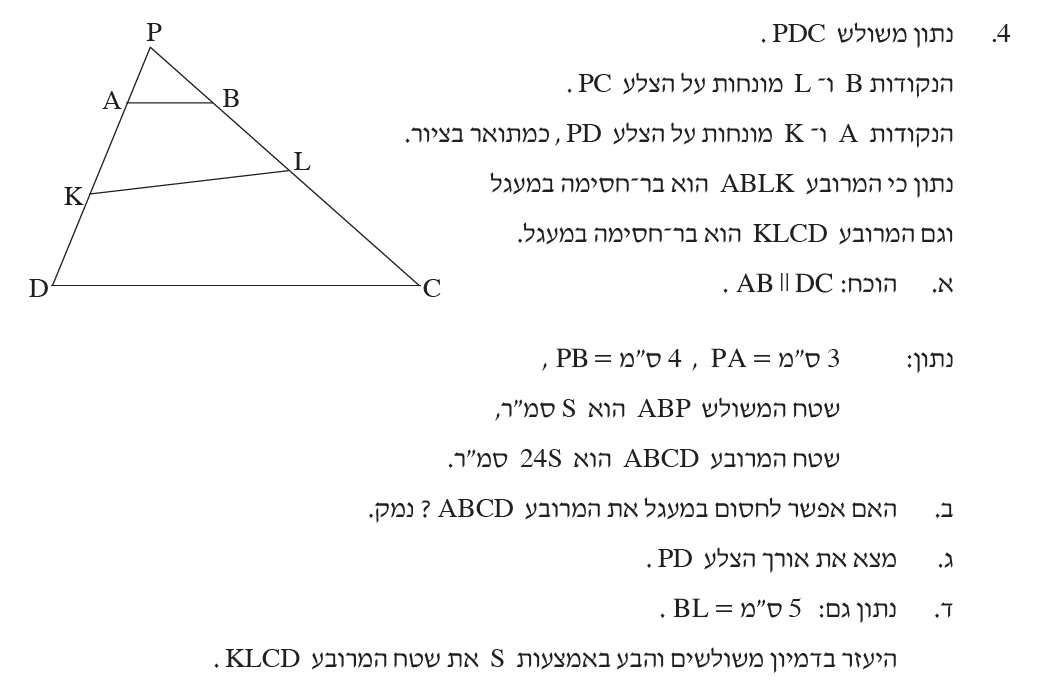
\includegraphics[width=\textwidth]{summer-2016b-4}
\end{center}
\vspace{-7mm}
\textbf{סעיף א}

שני מרובעים חסומים והמשפט המתאים הוא משפט
$56$ 
"ניתן לחסום מרובע במעגל אם ורק אם סכום זוג זוויות נגדיות שווה ל-%
$180^\circ$".
נצייר את שני המעגלים החוסמים את המרובעים, ונבחר זוג זוויות נגדיות, למשל,
$\angle LKA,\angle ABL$,
במרובע
$ABLK$.
נסמן
$\angle LKA=\alpha$
ונשתמש בקיצור
$\alpha'=180^\circ-\alpha$
עבור הזווית הנגדית
$\angle ABL$.
לפי זוויות משלימות בנקודה
$B$,
$\angle ABP=\alpha$,
ובנקודה
$K$,
$\angle LKD=\alpha'$.
נפעיל שוב את משפט
$56$
כדי להסיק ש-%
$\angle LCD=\alpha$.
מכאן ש-%
$AB\|DC$
לפי זוויות מתאימות.
\vspace{-1mm}
\begin{center}
\selectlanguage{english}
\begin{tikzpicture}
%\clip (-1,-1.7) rectangle +(5,7.2);
\coordinate [label=left:$D$] (D) at (0,0);
\coordinate [label=right:$C$] (C) at (4,0);
\coordinate [label=above:$P$] (P) at (1.5,5);
\coordinate (K) at ($(D)!.25!(P)$);
\coordinate (L) at ($(C)!.35!(P)$);
\coordinate (A) at ($(D)!.75!(P)$);
\draw[thick,name path=pd] (P) -- (D);
\draw[thick,name path=pc] (P) -- (C);
\path[name path=ab] (A) -- +(2,0);
\path[name intersections={of=ab and pc,by={B}}];
\draw[thick] (D) -- (C);
\draw[thick] (K) -- (L);
\draw[thick] (A) -- (B);
\tkzCircumCenter(A,B,L)\tkzGetPoint{O1}
\tkzDrawCircle[dashed,name path=circ1](O1,A)
\tkzCircumCenter(K,L,C)\tkzGetPoint{O2}
\tkzDrawCircle[dashed,name path=circ2](O2,L)
\fill (P) circle(1.5pt);
\fill (C) node[above left,xshift=-2pt] {$\alpha$} circle(1.5pt);
\fill (D) node[above right,xshift=2pt] {$\beta$} circle(1.5pt);
\fill (K) node[left,xshift=-6pt] {$K$} node[above right,xshift=2pt] {$\alpha$} node[below right,xshift=0pt,yshift=4pt] {$\alpha'$}  circle(1.5pt);
\fill (L) node[right,xshift=6pt] {$L$} node[left,xshift=-4pt,yshift=4pt] {$\beta$} node[below left,xshift=2pt,yshift=-2pt] {$\beta'$} circle(1.5pt);
\fill (A) node[left,xshift=-6pt] {$A$} node[below right,xshift=-4pt] {$\beta'$}  node[above right,xshift=0pt] {$\beta$} circle(1.5pt);
\fill (B) node[below left,xshift=2pt] {$\alpha'$} node[above left,xshift=-3pt] {$\alpha$} node[right,xshift=6pt] {$B$} circle(1.5pt);
\end{tikzpicture}
\end{center}

\np

\textbf{סעיף ב}

כדי להפעיל שוב את משפט
$56$
נצטרך להוכיח שהזוויות הנגדיות במרובע
$ABCD$
מקיימות
$\angle BAD+\angle BCD=180, \angle ADC+\angle ABC=180$.
נסמן
$\angle ADC=\beta$.

הוכחנו ש-%
$AB\|DC$,
ולפי זוויות חד-מתאימות בנקודות
$A,D$
ו-%
$B,C$,
וזוויות משלימות בנקודות
$A,B$,
נקבל
$\angle PAB=\angle ADC=\beta$,
$\angle PBA=\angle BCD=\alpha$.

אם המרובע 
$ABCD$
בר חסימה,
$\alpha'+\beta=180-\alpha+\beta=180$,
כך ש-%
$\alpha=\beta$,
אבל נתון ש-%
$PA\neq PB$.
המסקנה היא שלא ניתן לחסום את המרובע
$ABCD$.

\vspace{2ex}

\textbf{סעיף ג}

$\triangle PAB \sim \triangle PDC$
לפי ז.ז. אולם, זה לא עוזר: אמנם נתון היחס בין
$PA,PB$,
אבל יש שני זוגות של נעלמים
$PD,PC$
ו-%
$AB,DC$.
מה שכן ניתן הוא שטחים של שני המושלים, ולפי משפט
$100$
ז "יחס הצלעות הוא השורש של יחס השטחים", נכול לחשב את יחס הצלעות:
\[
\frac{PA}{PD}=\sqrt{\frac{S_{ABP}}{S_{PDC}}} = \sqrt{\frac{S_{ABP}}{S_{ABP} + S_{ABCD}}}=\sqrt{\frac{S}{S+24S}}=\frac{1}{5}\,.
\]
האורך של 
$PD$
הוא
$5\cdot PA=15$.

\vspace{2ex}

\textbf{סעיף ד}

מהזוויות שחישבנו ורשמנו באיור,
$\triangle PBA \sim \triangle PKL$
לפי ז.ז. יחס השטחים מתקבל מיחס אורכי הצלעות הנתונים ושחישבנו:
\[
\erh{12pt}
\begin{array}{l}
\displaystyle\frac{S_{PBA}}{S_{PKL}}=\left(\frac{PA}{PL}\right)^2=\left(\frac{3}{9}\right)^2=\frac{1}{9}\\
S_{KLCD}=S_{PDC}-S_{PKL}=25S-9S=16S\,.
\end{array}
\]
\vspace{-3ex}
\begin{center}
\selectlanguage{english}
\begin{tikzpicture}
\coordinate [label=left:$D$] (D) at (0,0);
\coordinate [label=right:$C$] (C) at (4,0);
\coordinate [label=above:$P$] (P) at (1.5,5);
\coordinate (K) at ($(D)!.25!(P)$);
\coordinate (L) at ($(C)!.35!(P)$);
\coordinate (A) at ($(D)!.75!(P)$);
\draw[thick,name path=pd] (P) -- (D);
\draw[thick,name path=pc] (P) -- (C);
\path[name path=ab] (A) -- +(2,0);
\path[name intersections={of=ab and pc,by={B}}];
\draw[thick] (D) -- (C);
\draw[thick] (K) -- (L);
\draw[thick] (A) -- (B);
\fill (P) circle(1.5pt);
\fill (C) circle(1.5pt);
\fill (D) circle(1.5pt);
\fill (K) node[left,xshift=-6pt] {$K$} node[above right] {$\alpha$} circle(1.5pt);
\fill (L) node[right,xshift=6pt] {$L$} node[left,xshift=-4pt,yshift=4pt] {$\beta$}  circle(1.5pt);
\fill (A) node[left,xshift=-6pt] {$A$} node[above right] {$\beta$} circle(1.5pt);
\fill (B) node[above left,xshift=-3pt] {$\alpha$} node[right,xshift=6pt] {$B$} circle(1.5pt);
\path (B) -- node[right] {$4$} (P);
\path (L) -- node[right] {$5$} (B);
\path (A) -- node[left] {$3$} (P);
\end{tikzpicture}
\end{center}


%%%%%%%%%%%%%%%%%%%%%%%%%%%%%%%%%%%%%%%%%%%%%%%%%%%%%%%%%%%%%%%%%%%


\np

\section{קיץ תשע"ו מועד א}

\begin{center}
\selectlanguage{english}
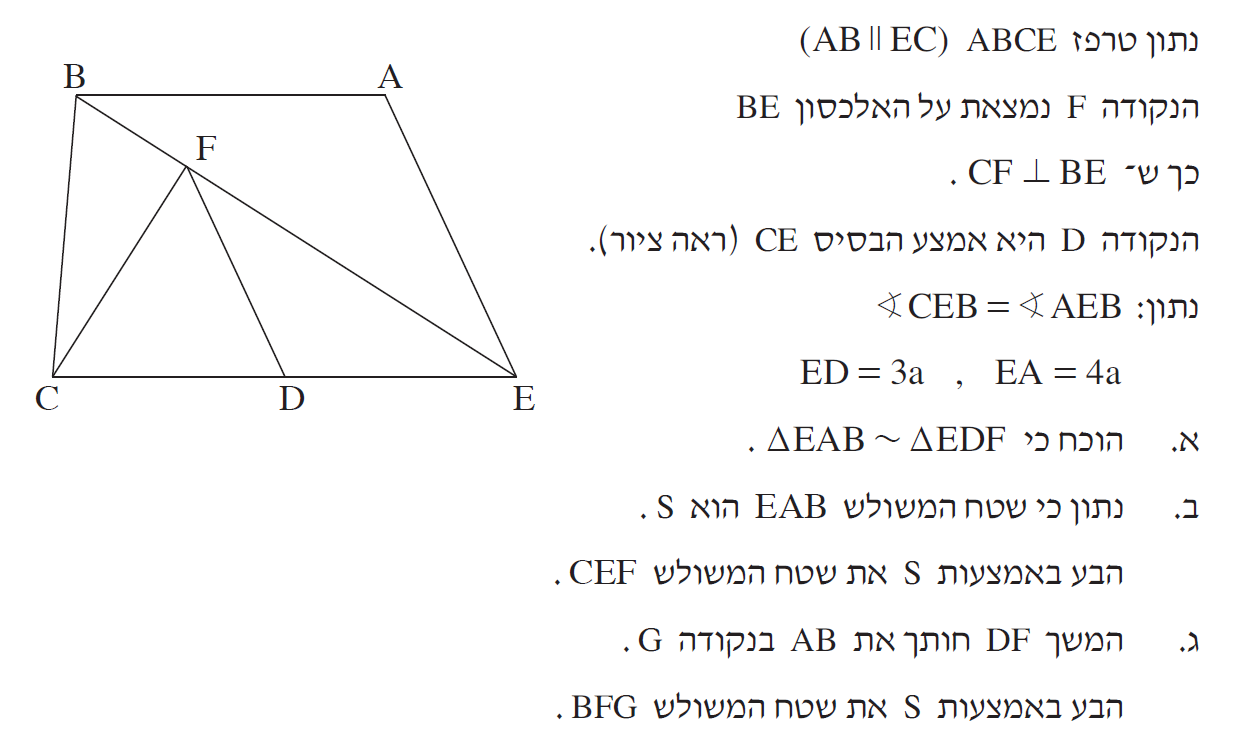
\includegraphics[width=\textwidth]{summer-2016a-4}
\end{center}

\textbf{סעיף א}

נסמן את הזוויות
$\angle AEB=\angle CEB=\alpha$
ונמסן את האורכים הנתונים. כעת קופץ לעין משפט
$86$
"במשולש ישר זווית התיכון ליתר שווה למחצית היתר", ולכן
$DF=CD=DE$,
ו-%
$\triangle EDF$
שווה שוקיים, 
$\angle DFE=\alpha$.
כמו כן, נתון ש-%
$AB\|EC$,
כך ש-%
$\angle ABE=\alpha$
לפי זוויות מתחלפות עם
$\angle CEB$. 
לפי ז.ז.
$\triangle EDF \sim \triangle EAB$.
\vspace{-10mm}
\begin{center}
\selectlanguage{english}
\begin{tikzpicture}[scale=.8]
\coordinate [label=above right:$A$] (A) at (6.5,4.5);
\coordinate [label=above left:$B$] (B) at (.5,4.5);
\coordinate [label=below right:$E$] (E) at (10,0);
\coordinate [label=below left:$C$] (C) at (0,0);
\coordinate [label=below:$D$] (D) at (5,0);
\coordinate [label=above right:$F$] (F) at ($(B)!(C)!(E)$);
\fill (A) circle(1.5pt);
\fill (B) node[below right,xshift=18pt] {$\alpha$} circle(1.5pt);
\fill (C) circle(1.5pt);
\fill (D) circle(1.5pt);
\fill (E) node[above left,xshift=-18pt,yshift=-1pt] {$\alpha$} node[above left,xshift=-14pt,yshift=12pt] {$\alpha$} circle(1.5pt);
\fill (F) node[below right,xshift=14pt,yshift=-11pt] {$\alpha$} circle(1.5pt);
\draw[thick] (A) -- (B) -- (C) -- (E) -- cycle;
\draw[thick] (B) -- (E);
\draw[thick] (C) -- (F) -- (D);
\path[name path=cf] (C) -- ($ (C) ! 1.8 ! (F) $);
\path[name path=ab] (A) -- (B);
%\path [name intersections={of=cf and ab,by={G}}];
%\fill (G) node[above] {$G$} circle(1.5pt);
%\draw[thick] (F) -- (G);
\draw[rotate=-114] (F) rectangle +(7pt,7pt);
\path (C) -- node[below,yshift=-2pt] {$3a$} (D);
\path (A) -- node[right,xshift=2pt] {$4a$} (E);
\path (D) -- node[below,yshift=-2pt] {$3a$} (E);
\path (F) -- node[left,yshift=0pt] {$3a$} (D);
\draw[thick,dashed] (F) -- ($ (C)!(F)!(D) $) coordinate(H);
\draw (H) rectangle +(7pt,7pt);
\end{tikzpicture}
\end{center}

\np

\textbf{סעיף ב}

כדי לחשב את השטח של 
$\triangle CEF$
יש לנו בסיס
$CE$
ונבנה גובה מ-%
$F$
ל-%
$CE$.
חדי עין ישימו לב גובה זה משותף לשני המשולשים
$\triangle CFD,\triangle DFE$.
הבסיסים
$CD=DE=3a$
שווים, ולכן השטחים של שני המשולים שווים.

בסעיף א הוכחנו ש-%
$\triangle CEB\sim AEB$,
לפי משפט
$100$%
ז "יחס השטחים שווה לריבוע יחס הדמיון":
\[
\erh{12pt}
\begin{array}{l}
\displaystyle\frac{S_{DFE}}{S_{EAB}}= \left(\frac{DE}{AE}\right)^2= \left(\frac{3a}{4a}\right)^2=\frac{9}{16}\\
S_{CEF} = S_{CFD}+S_{DFE}=2 \, S_{DFE}= \frac{9}{8}\, S\,.
\end{array}
\]

\textbf{סעיף ג}

אנחנו צריכים לחשב את האורך של צלע של
$\triangle BFG$
כדי לחשב את יחס השטחים. כבר הראינו ש-%
$\angle ABE = \angle BEC=\alpha$
ו-%
$\angle BFG = \angle DFE=\alpha$
הן זוויות קודקודיות. לכן
$\triangle BFG \sim \triangle DFE$
לפי ז.ז. הזווית
$\angle AGD=2\alpha$
לפי משפט
$13$
"זווית חיצונית למשולש שווה לסכום שתי הזוויות הפנימיות שאינן צמודות לה". המרובע
$AGDE$
הוא מקבילית לפי משפט
$29$
"מרובע שבו כל זוג זוויות נגדיות שוות הוא מקבילית". 
$GD=GF+FD$
וכעת ניתן לחשב את
$GF$:
\[
GF=GD-DF=AE-DF=4a-3a=a\,,
\]
ולהשתמש שוב במשפט
$101$%
ז:
\[
\erh{6pt}
\begin{array}{l}
\displaystyle\frac{S_{BFG}}{S_{DFE}}=\left(\frac{a}{3a}\right)^2=\frac{1}{9}\\\\
\displaystyle S_{BFG}=\frac{1}{9}S_{DFE}=\frac{1}{9}\cdot\frac{1}{2}S_{CEF}=\frac{1}{(9\cdot 2)}\frac{9}{8}S=\frac{1}{16}S\,.
\end{array}
\]

\vspace{-10ex}

\begin{center}
\selectlanguage{english}
\begin{tikzpicture}[scale=.8]
\coordinate [label=above right:$A$] (A) at (6.5,4.5);
\coordinate [label=above left:$B$] (B) at (.5,4.5);
\coordinate [label=below right:$E$] (E) at (10,0);
\coordinate [label=below left:$C$] (C) at (0,0);
\coordinate [label=below:$D$] (D) at (5,0);
\coordinate (F) at ($(B)!(C)!(E)$);
\fill (A)  node[below left] {$180-2\alpha$}circle(1.5pt);
\fill (B) node[below left,xshift=-8pt,yshift=-8pt] {$\alpha$} circle(1.5pt);
\draw[<-] (1.1,4.4) -- +(-155:26pt);
\draw[<-] (1.4,4.2) -- +(-170:33pt);
\fill (C) circle(1.5pt);
\fill (D) node[above left,xshift=-4pt] {$2\alpha$} node[above right,xshift=-4pt] {$180-2\alpha$} circle(1.5pt);
\fill (E) node[above left,xshift=-18pt,yshift=-1pt] {$\alpha$} node[above left,xshift=-14pt,yshift=12pt] {$\alpha$}  circle(1.5pt);
\fill (F) node[below left,xshift=4pt,yshift=-4pt] {$F$} node[below right,xshift=16pt,yshift=-12pt] {$\alpha$} circle(1.5pt);
\draw[thick] (A) -- (B) -- (C) -- (E) -- cycle;
\draw[thick] (B) -- (E);
\draw (D) -- (F);
%\draw[thick] (F) -- (C);
\path[name path=df] (D) -- ($ (D) ! 1.8 ! (F) $);
\path[name path=ab] (A) -- (B);
\path [name intersections={of=df and ab,by={G}}];
\fill (G) node[above] {$G$} node[below right,xshift=8pt] {$2\alpha$} circle(1.5pt);
\draw[thick] (F) -- (G);
%\draw[rotate=-114] (F) rectangle +(7pt,7pt);
%\path (C) -- node[below,yshift=-2pt] {$3a$} (D);
\path (A) -- node[right,xshift=2pt] {$4a$} (E);
\path (D) -- node[below,yshift=-2pt] {$3a$} (E);
\path (F) -- node[left,yshift=0pt] {$3a$} (D);
%\draw[thick,dashed] (F) -- ($ (C)!(F)!(D) $) coordinate(H);
%\draw (H) rectangle +(7pt,7pt);
\end{tikzpicture}
\end{center}

%%%%%%%%%%%%%%%%%%%%%%%%%%%%%%%%%%%%%%%%%%%%%%%%%%%%%%%%%%%%%%%%%%%

\np


\section{חורף תשע"ו}

\begin{center}
\selectlanguage{english}
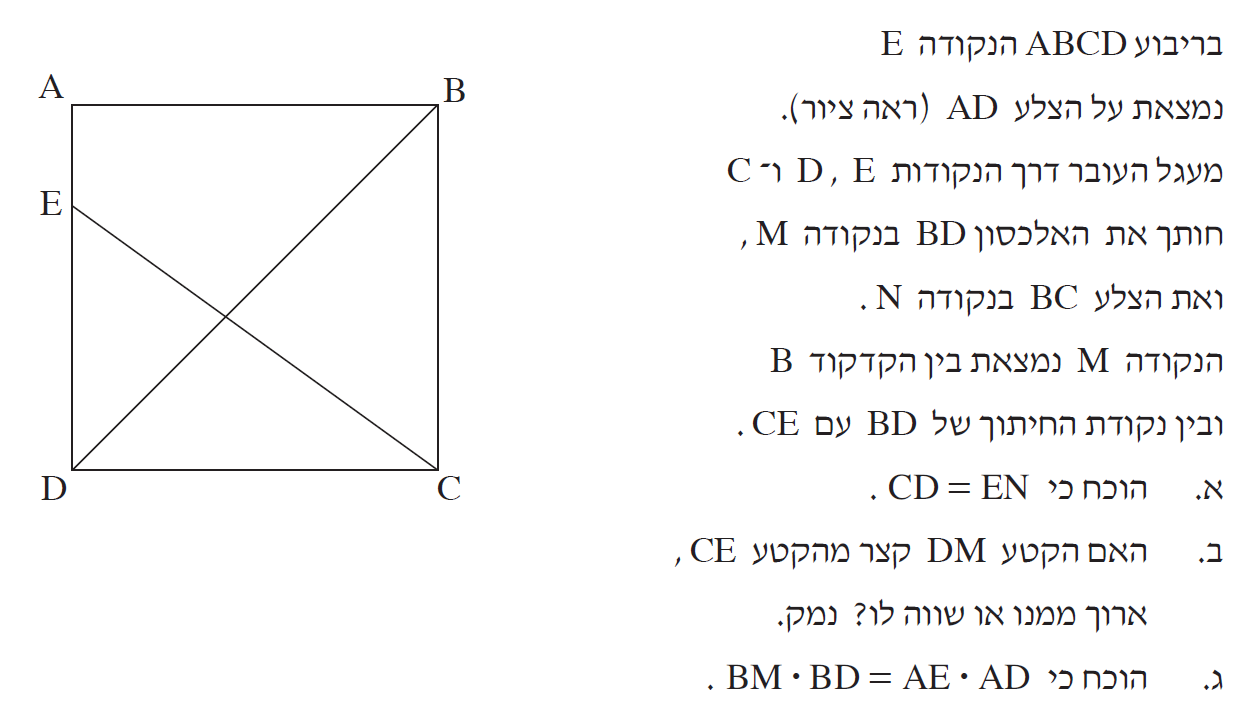
\includegraphics[width=.9\textwidth]{winter-2016-4}
\end{center}

\vspace{-2mm}

\textbf{סעיף א}

קשה להבין את השאלה אלא אם מציירים תרשים חדש עם הנקודות 
$M,N$
והקו
$EN$.
המעגל מוגדר כך שהוא עובר דרך הנקודות
$C,D,E$,
ונתון גם שהנקודה
$N$
נמצאת על המעגל. מכאן ש-%
$ENDC$
הוא מרובע הסום במעגל. נשתמש במשפט 
$56$
"ניתן לחסום מרובע במעגל אם ורק אם סכום זוג זוויות נגדיות שווה ל-%
$180^\circ$".
$ABCD$
הוא ריבוע כך ש-%
$\angle ADC=\angle EDC=90^\circ$,
$\angle BCD=\angle NCD=90^\circ$.
לפי המשפט:
\[
\angle ENC=180-\angle EDC=90,\quad \angle NED=180-\angle NCD=90\,.
\]
מרובע שכל הזוויות שלו ישרות הוא מלבן ו-%
$CD=EN$.

\begin{center}
\selectlanguage{english}
\begin{tikzpicture}[scale=.85]
\coordinate [label=above left:$A$] (A) at (0,5);
\coordinate [label=above right:$B$] (B) at (5,5);
\coordinate [label=below right:$C$] (C) at (5,0);
\coordinate [label=below left:$D$] (D) at (0,0);
\coordinate [label=left:$E$] (E) at (0,3.5);
\draw[thick] (A) -- (B) -- (C) -- (D) -- cycle;
\draw[thick,name path=db] (D) -- (B);
\draw[thick,name path=ce] (C) -- (E);
\fill (A) circle(1.5pt);
\fill (B) circle(1.5pt);
\fill (C) circle(1.5pt);
\fill (D) circle(1.5pt);
\fill (E) circle(1.5pt);
\tkzCircumCenter(C,D,E)\tkzGetPoint{O}
\tkzDrawCircle[thick,name path=circ](O,C)
\path [name intersections={of=db and ce,by={F}}];
%\fill (F) node[above,yshift=4pt] {$F$} circle(1.5pt);
\path [name intersections={of=circ and db,by={M}}];
\fill (M) node[left,xshift=-4pt] {$M$} circle(1.5pt);
\path[name path=bc] (B) -- (C);
\path [name intersections={of=circ and bc,by={N}}];
\fill (N) node[right] {$N$} circle(1.5pt);
\draw[thick,dashed] (E) -- (N);
\draw[rotate=0] (D) rectangle +(7pt,7pt);
\draw[rotate=90] (C) rectangle +(7pt,7pt);
\end{tikzpicture}
\end{center}

\np

הוכחה אחרת משתמשת במשפט
$74$
"זווית היקפית בת 
$90^\circ$
נשענת על קוטר". הנקודות
$C,D,E,N$
נמצאות על מעגל, 
$\angle EDC=90^\circ$,
כך ש-%
$EC$
הוא קוטר לפי משפט
$74$
"זווית היקפית בת
$90^\circ$
נשענת על קוטר". לפי המשפט ההפוך
$(73)$
$\angle ENC=90^\circ$.
כדי להשלים את סכום הזוויות במרובע ל-%
$360^\circ$,
$\angle NED$
חייב להיות 
$90^\circ$
ו-%
$ENDC$
הוא מלבן.


\textbf{סעיף ב}

בזבזתי הרבה זמן בנסיונות לפתור סעיף זה כי חשבתי להשוות אורכים לפי משולשים דומים או משפט פיתגורס. לבסוף נזכרתי במשפט
$66$
"במעגל, אם מרחקו של מיתר ממרכז המעגל קטן יותר ממרחקו של מיתר אחר, אז מיתר זה ארוך יותר מהמיתר האחר". בהוכחה השנייה לסעיף א ראינו ש-%
$EC$
הוא קוטר, וקוטר הוא מיתר הקרוב ביותר למרכז המעקל )עובר דרכו( ולכן הוא ארוך יותר מכל מיתר שאינו קוטר. מה שנשאר לעשות הוא להוכיח ש-%
$DM$
אינו קוטר.

נתון שהנקודה
$M$
נמצאת בין 
$B$
לבין נקודת החיתוך המסומן ב-%
$F$.
נתון גם ש-%
$E$
נמצאת על
$AD$
ונניח שהכוונה היא ש-%
$E$
שונה מנקודות הקצה
$A,D$.
הוכחנו ש-%
$EN\|AB$
ולכן אם 
$E$
שונה מ-%
$A$
גם
$N$
שונה מ-%
$B$,
ו-%
$M$
אינה מתלכדת עם
$N$.
\vspace{-4mm}

\begin{center}
\selectlanguage{english}
\begin{tikzpicture}[scale=.85]
\coordinate (A) at (0,5);
\coordinate (B) at (5,5);
\coordinate [label=below right:$C$] (C) at (5,0);
\coordinate [label=below left:$D$] (D) at (0,0);
\coordinate [label=left:$E$] (E) at (0,3.5);
\draw[thick,name path=db] (D) -- (B);
\draw[thick,name path=ce] (C) -- (E);
\fill (A) node[above left] {$A$} circle(1.5pt);
\fill (B) node[above right] {$B$} circle(1.5pt);
\fill (C) circle(1.5pt);
\fill (D) circle(1.5pt);
\fill (E) circle(1.5pt);
\tkzCircumCenter(C,D,E)\tkzGetPoint{O}
\tkzDrawCircle[thick,name path=circ](O,C)
\path [name intersections={of=db and ce,by={F}}];
\fill (F) node[above,yshift=4pt] {$F$} circle(1.5pt);
\path [name intersections={of=circ and db,by={M}}];
\fill (M) node[left,xshift=-4pt] {$M$} circle(1.5pt);
\path[name path=bc] (B) -- (C);
\path [name intersections={of=circ and bc,by={N}}];
\fill (N) node[right] {$N$} circle(1.5pt);
\draw[thick,dashed] (D) -- (N);
\draw[rotate=0] (D) rectangle +(7pt,7pt);
\draw[rotate=90] (C) rectangle +(7pt,7pt);
\fill (O) node[below,yshift=-4pt] {$O$} circle(1.5pt);
\draw[thick] (B) -- (A) -- (D) -- (C) -- (N) -- (B) -- (D);
\draw[thick,dashed] (E) -- (N);
\end{tikzpicture}
\end{center}

%\np

\vspace{-30mm}

\textbf{סעיף ג}

הנטייה הראשונה היא להשתמש במשפט תאלס, אבל משפט זה מנוסח כחילוק ולא ככפל על קטעים של אותו קן. המשפט שמנוסח בכפל הוא משפט
$102$
"אם מנקודה מחוץ למעגל יוצאים שני חותכים, אז מכפלת חותך אחד בחלקו החיצוני שווה למכפלת החותך השני בחלקו החיצוני". נשתמש במשפט זה עבור החותכים
$BC,BD$
היוצאים מנקודה
$B$
ונקבל
$BM\cdot BD = BN \cdot BC$.

$AD=BC$
כי הם צלעות בריבוע 
$ABCD$,
ו-%
$ED=NC$
כי הם צעלות של
$ENCD$
שהוכחנו בסעיף א שהוא מלבן. מכאן:
\[
BM\cdot BD =  BN \cdot BC = (BC-NC)\cdot BD = (AD-ED) \cdot AD = AE\cdot AD\,.
\]


%%%%%%%%%%%%%%%%%%%%%%%%%%%%%%%%%%%%%%%%%%%%%%%%%%%%%%%%%%%%%%%%%%%

\np


\section{קיץ תשע"ה מועד ב}

\begin{center}
\selectlanguage{english}
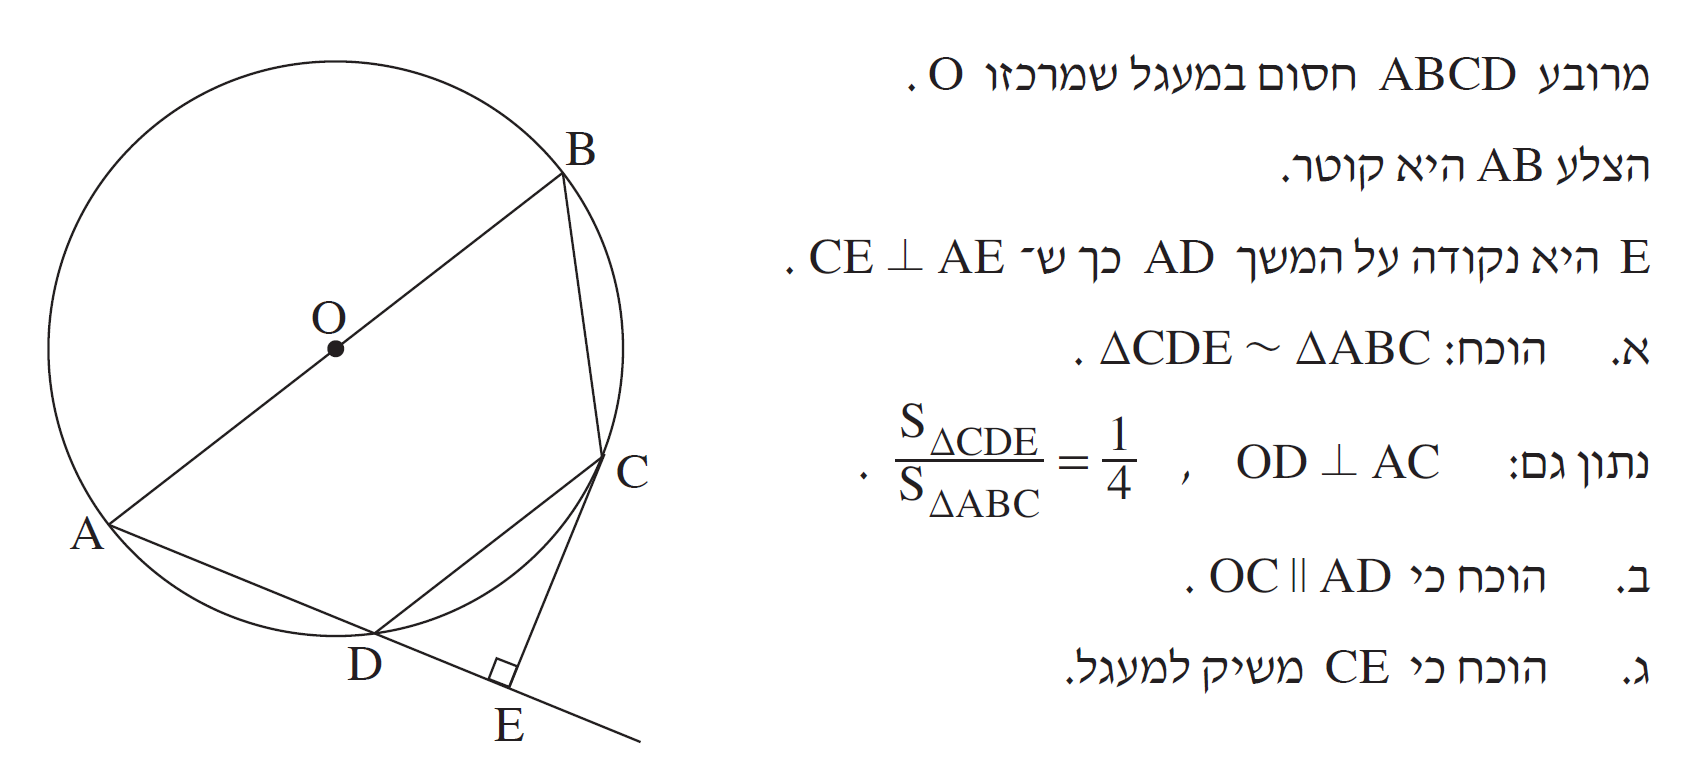
\includegraphics[width=\textwidth]{summer-2015b-4}
\end{center}

\textbf{סעיף א}

מרובע חסום במעגל מכוון למשפט
$56$
"ניתן לחסום מרובע במעגל אם ורק אם סכום זוג זוויות נגדיות שווה ל-%
$180^\circ$". 
נתון גם שצלע שלו הוא קוטר והמשפט ררלוונטי הוא
$73$
"זווית היקפית הנשענת על קוטר היא זווית ישרה 
$(90^\circ)$".
כדי לקבל את המשלוש
$\triangle ABC$,
נצייר את הקו
$AC$

ו-%
$\angle ACB=90^\circ$
כי הוא נשען על קוטר. 

נסמן זוויות לפי משפט
$(56)$:
$\angle ABC=\alpha$,
$\angle BAC=180-\alpha=\alpha'$.
לפי זוויות משלימות בנקודה
$D$,
$\angle CDE=180-\alpha'=\alpha=\angle ABC$,
ו-%
$\triangle CDE \sim \triangle ABC$
לפי ז.ז.


\begin{center}
\selectlanguage{english}
\begin{tikzpicture}[scale=.9]
\coordinate [label=above:$O$] (O) at (0,0);
\coordinate [label=below left:$A$] (A) at (-2,-2);
\fill (O) circle(1.5pt);
\fill (A) circle(1.5pt);
\node [draw,thick,circle through=(A),name path=circ] (circle) at (O) {};
\path [name path=diam] (A) -- +(45:6);
\path [name intersections={of=circ and diam,by={B}}];
\fill (B) node[above right] {$B$} node[below,xshift=-3pt,yshift=-6pt] {$\alpha$} circle(1.5pt);
\draw[thick] (A) -- (B);
\draw [thick,name path=ad] (A) -- +(-15:5);
\path [name intersections={of=circ and ad,by={dummy1,D}}];
\fill (D) node[below] {$D$} node[right,xshift=10pt,yshift=1pt] {$\alpha?$} node[above,xshift=0pt,yshift=0pt] {$\alpha'$} circle(1.5pt);
\path [thick,name path=dc] (D) -- +(45:4);
\path [name intersections={of=circ and dc,by={dummy2,C}}];
\fill (C) node[right] {$C$} circle(1.5pt);
\draw [thick] (D) -- (C) -- (B);
\coordinate (E) at ($(A)!(C)!(D)$);
\fill (E)  node[below] {$E$} circle(1.5pt);
\draw[thick] (C) -- (E);
\draw[rotate=76] (E) rectangle +(5pt,5pt);
\draw[thick,dashed] (A) -- (C);
\draw[rotate=108] (C) rectangle +(5pt,5pt);
\end{tikzpicture}
\end{center}

\np

\textbf{סעיף ב}

בתרשים נראה שהמרובע
$AODC$
הוא מקבילית, ואם כן, 
$OC\|AD$.
נתון גם ש-%
$OD\perp AC$,
כך שאם המרובע הוא מקבילית, הוא גם מעוין לפי משפט
$36$
"מקבילית שבה האלכסונים מאונכים זה לזה היא מעוין". למעשה לא צריך להשתמש במשפט
$36$
כדי להוכיח שהמקבילית היא מעוין כי 
$OA=OC=r$.
מכאן שסביר יותר שהנתון
$OD\perp AC$
יעזור להוכיח ש-%
$AODC$
הוא מקבילית.

כעת נפנה לנתון על יחס השטחים של המשולשים. לפי משפט
$100$%
ז "יחס השטחים שווה לריבוע יחס הדמיון", היחס הצלעות במשולשים הדומים הוא
$\sqrt{\frac{1}{4}}=\frac{1}{2}$.
מכאן ש-%
$CD=\frac{1}{2}AB=\frac{1}{2}\cdot 2r=r$.
אם נוכיח ש-%
$AD=r$
יהיה לנו את המקבילית )מעוין( שנחוץ כדי להוכיח ש-%
$OC\|AD$.

נחזור לנתון
$OD\perp AC$.
הוכחנו ש-%
$\triangle OCD$
הוא שווה שוקיים )למעשה הוא שווה צלעות(, כך ש-%
$CA$
הוא גובה ל-%
$OD$,
ולפי משפט
$6$
"במשולש שווה שוקיים , חוצה זווית הראש, התיכון לבסיס והגובה לבסיס מתלכדים", ולכן
$OF=FD=\frac{r}{2}$
ו-%
$\triangle OCF\cong\triangle DCF$.\footnote{%
החפיפה נובעת ממשפט 
$20$
"משפט חפיפה שתי צלעות והזווית שמול הצלע הגדולה מבין השתיים" לאחר שנטען שהזווית הישרה גדולה יותר מהזוויות האחרות. בספרי גיאומטריה משתמשים במשפט זה כך: שני משלושים ישר זווית חופפים עם היתר וצלע אחר שווים.%
}
אותה הוכחה מראה ש-%
$\triangle OAF\cong \triangle OCF$
ו-%
$\triangle DAF\cong \triangle OAF$.
מכאן ש-%
$AD=OA=r$.
\begin{center}
\selectlanguage{english}
\begin{tikzpicture}[scale=.9]
\coordinate [label=above:$O$] (O) at (0,0);
\coordinate [label=below left:$A$] (A) at (-2,-2);
\fill (O) circle(1.5pt);
\fill (A) circle(1.5pt);
\node [draw,thick,circle through=(A),name path=circ] (circle) at (O) {};
\path [name path=diam] (A) -- +(45:6);
\path [name intersections={of=circ and diam,by={B}}];
\fill (B) node[above right] {$B$} circle(1.5pt);
\draw[thick] (A) -- (B);
\draw [thick,name path=ad] (A) -- +(-15:5);
\path [name intersections={of=circ and ad,by={dummy1,D}}];
\fill (D) node[below] {$D$} circle(1.5pt);
\path [thick,name path=dc] (D) -- +(45:4);
\path [name intersections={of=circ and dc,by={dummy2,C}}];
\fill (C) node[right] {$C$} circle(1.5pt);
\draw [thick] (D) -- node[above] {$r$} (C) -- (B);
\coordinate (E) at ($(A)!(C)!(D)$);
\fill (E)  node[below] {$E$} circle(1.5pt);
\draw[thick] (C) -- (E);
\draw[rotate=76] (E) rectangle +(5pt,5pt);
\draw[thick,dashed,name path=ac] (A) -- (C);
\draw[rotate=107] (C) rectangle +(5pt,5pt);
\draw[thick,dashed,name path=od] (D) -- node[left,near end,yshift=-2pt] {$r/2$} node[left,near start,yshift=-2pt] {$r/2$} (O) -- node[above] {$r$} (C);
\path [name intersections={of=ac and od,by={F}}];
\fill (F) node[above right] {$F$} circle(1.5pt);
\draw[rotate=107] (F) rectangle +(5pt,5pt);
\path (A) -- node[above] {$r$} (O) -- node[above] {$r$} (B);
\path (A) -- node[below,yshift=-14pt] {$r?$} (D);
\draw[<-] ($(A) !.5 ! (D) $) -- +(0,-16pt);
\end{tikzpicture}
\end{center}
בפתרונות אחרים שראיתי, משתמשים בעובדה ש-%
$\triangle OCD$
הוא שווה צלעות שהזוויות שלו הן
$60^\circ$.
לא מצאתי שערך זה נחוץ כדי להוכיח את הטענה.

\vspace{2ex}
\textbf{סעיף ג}

המשפט היחיד שהמסקנה שלו היא שקו הוא משיק הוא משפט
$78$
"ישר המאונך לרדיוס בקצהו הוא משיק למעגל", כאן
$CE\perp OC$.
כאן כן נשתמש בעובדה ש-%
$\triangle OCD,\triangle OAD$
הם שווה צלעות ו-%
$\angle OCD=\angle OAD=60^\circ$.
בסעיף א הוכחנו ש-%
$\triangle ABC\sim \triangle CDE$,
כך ש-%
$\angle CAB = \angle ECD$.
בסעיף ב הוכחנו ש-%
$AC$
הוא חוצה זווית של
$\angle OAD$.
מכאן ש-%
\[
\angle ECO = \angle ECD + \angle OCD = \angle CAB + 60^\circ = \frac{1}{2}\angle OAD + 60^\circ=\frac{1}{2}\cdot 60^\circ + 60^\circ = 90^\circ\,.
\]


%%%%%%%%%%%%%%%%%%%%%%%%%%%%%%%%%%%%%%%%%%%%%%%%%%%%%%%%%%%%%%%%%%%
\np


\section{קיץ תשע"ה מועד א}

\begin{center}
\selectlanguage{english}
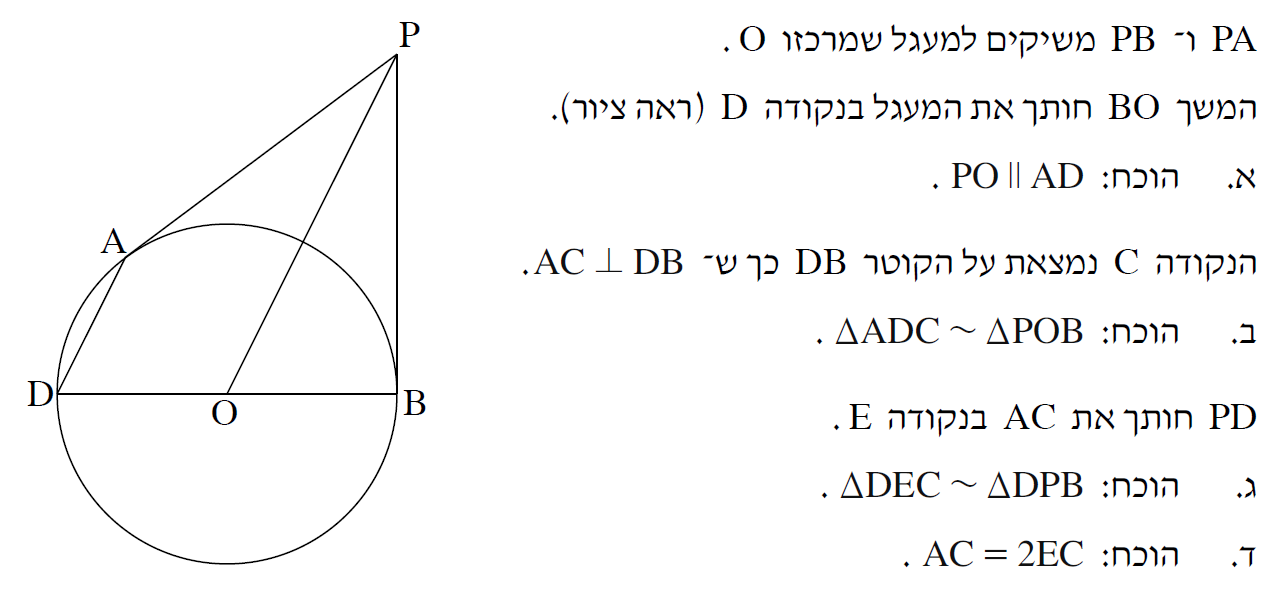
\includegraphics[width=\textwidth]{summer-2015a-4}
\end{center}

\vspace{-2ex}
\textbf{סעיף א}


כאשר יש שני משיקים וקו מהנקודת החיתוך של המשיקים למרכז המעגל המשפטים האלה עשויים להיות קלוונטיים: משפט
$(77)$
"המשיק למעגל מאונך לרדיוס בנקודת ההשקה", משפט
$(80)$
"שני משיקים למעגל היוצאים מאותה נקודה שווים זה לזה", ומשפט
$(81)$
"קטע המחבר את מרכז המעגל לנקודה ממנה יוצאים שני משיקים למעגל, חוצה את הזווית שבין המשיקים". באיור, הוספנו סימנים המציגים את המשפטים האלה. 

ניתן להשלים את שאר הזוויות, כאשר השתמשנו בקיצור
$\alpha' = 90^\circ-\alpha$,
תוך שימוש בעובדות שסכום הזוויות במשולש הוא
$180^\circ$,
וסכום הזוויות המשלימות לזווית שטוחה הוא
$180^\circ$.
משוויון הרדיוסים נקבל ש-%
$\triangle AOD$
הוא שווה שוקיים, ולכן
$\angle ADO=\angle DAO=\alpha'$.
מכאן ש-%
$\angle ADO=\angle POB=\alpha'$
ו-%
$PD\|AD$
לפי זוויות מתאימות.

\begin{center}
\selectlanguage{english}
\begin{tikzpicture}[scale=.9]
\coordinate [label=below:$O$] (O) at (0,0);
\coordinate [label=right:$B$] (B)  at (2.5,0);
\coordinate [label=above right:$P$] (P) at (2.5,4.5);
\node [draw,thick,circle through=(B),name path=circ] (circle) at (O) {};
\draw[thick,name path=tan1] (P) --  node[right] {$a$} (B);
\path[name path=bd] (B) -- +(-5.2,0);
\path [name intersections={of=circ and bd,by={dummy,D}}];
\draw[thick] (B)--node[below] {$r$} (O);
\draw[thick] (O) -- node[below] {$r$} (D);
\coordinate (A) at (tangent cs:node=circle,point={(P)},solution=1);
\draw[thick] (P) -- node[above] {$a$} (A) -- (D);
\fill (O) node[above right,yshift=-2pt,xshift=2pt] {$\alpha'$} node[above,yshift=6pt,xshift=1pt] {$\alpha'$} node[above left,yshift=-2pt,xshift=-4pt] {$2\alpha$} circle(1.5pt);
\fill (B) circle(1.5pt);
\fill (P) node[below left,yshift=-16pt,xshift=-14pt] {$\alpha$} node[below,yshift=-17pt,xshift=-5pt] {$\alpha$} circle(1.5pt);
\fill (D) node[left] {$D$} node[above right,yshift=-2pt,xshift=2pt] {$\alpha'$} circle(1.5pt);
\fill (A) node[above left] {$A$} node[below,yshift=-6pt] {$\alpha'$} circle(1.5pt);
\draw[thick] (P) -- (O);
\draw[thick,dashed] (O) -- node[above right,xshift=-2pt] {$r$} (A);
\draw[rotate=-60] (A) rectangle +(5pt,5pt);
\draw[rotate=90] (B) rectangle +(5pt,5pt);
\end{tikzpicture}
\end{center}

\np

\textbf{סעיף ב}

הצעד הראשון הוא להוסיף לתרשים את הנקודה
$C$
ולסמן את הנתון ש-%
$AC\perp DB$.
הרבה זוויות מופיעות בתרשים ולכן ננסה להוכיח דמיון לפי ז.ז. מסעיף א אנו יודעים ש-%
$\angle ADC = \angle POB = \alpha'$,
ולכן עבור המשולשים ישר הזווית
$\triangle ADC \sim \triangle POB$.

\vspace{-2ex}
\begin{center}
\selectlanguage{english}
\begin{tikzpicture}[scale=.9]
\coordinate [label=below:$O$] (O) at (0,0);
\coordinate [label=right:$B$] (B)  at (2.5,0);
\coordinate [label=above right:$P$] (P) at (2.5,4.5);
\node [draw,thick,circle through=(B),name path=circ] (circle) at (O) {};
\draw[thick,name path=tan1] (P) -- (B);
\path[name path=bd] (B) -- +(-5.2,0);
\path [name intersections={of=circ and bd,by={dummy,D}}];
\draw[thick] (B)--(O);
\draw[thick] (O) -- (D);
\coordinate (A) at (tangent cs:node=circle,point={(P)},solution=1);
\draw[thick] (P) -- (A) -- (D);
\fill (O)  node[above right,yshift=-2pt,xshift=4pt] {$\alpha'$} circle(1.5pt);
\fill (B) circle(1.5pt);
\fill (P) node[below left,yshift=-18pt,xshift=-12pt] {$\alpha$} node[below,yshift=-18pt,xshift=-5pt] {$\alpha$} circle(1.5pt);
\fill (D) node[left] {$D$} node[above right,yshift=-2pt,xshift=12pt] {$\alpha'$} circle(1.5pt);
\fill (A) node[above left] {$A$} circle(1.5pt);
\draw[thick] (P) -- (O);
\draw[thick] (O) -- (A);
\draw[rotate=-60] (A) rectangle +(5pt,5pt);
\draw[rotate=90] (B) rectangle +(5pt,5pt);
\draw[thick,dashed,name path=ac] (A) -- ($(D)!(A)!(B)$) node[below] {$C$} coordinate (C);
\draw[rotate=90] (C) rectangle +(5pt,5pt);
\draw[thick,dashed,name path=pd] (P) -- (D);
\draw[thick] (-2,0) arc[start angle=0,end angle=72,radius=4mm];
\path [name intersections={of=pd and ac,by={E}}];
\fill (E) node[right,yshift=-2pt] {$E$} circle(1.5pt);=;
\end{tikzpicture}
\end{center}
\vspace{-2ex}

\textbf{סעיף ג}

נוסיף את הנקודה 
$E$
לתרשים. הזווית
$EDC$
של המשולש
$\triangle DEC$
היא למעשה אותה זווית
$PDB$
של המשולש
$\triangle DPB$,
ולכן
$\triangle DEC\sim \triangle DPB$
לפי ז.ז. במשולשים ישר זווית.

\textbf{סעיף ד}

עלינו לחפש ערך אחד שהוא כפול מערך אחר. כמובן הקוטר
$DB$
כפול מהרדיוסים
$DO,OB$.
בסעיפים הקודמים הוכחנו ששני זוגות של משולשים דומים. נפשט את האיור וננסה להוכיח את המשוואה תוך שימוש במשולשים. עבור 
$AC$,
מסעיף ב
$\triangle ADC \sim \triangle POB$,
ולכן:
\[
\frac{AC}{PB} = \frac{DC}{OB} = \frac{DC}{r}\,.
\]
מסעיף ג
$\triangle DEC \sim \triangle DPB$,
ולכן:
\[
\frac{EC}{PB} = \frac{DC}{DB} = \frac{DC}{2r}\,.
\]
נציב את
$PB\cdot DC$
ממשוואה אחת בשנייה ונקבל
$AC=2EC$.


\begin{center}
\selectlanguage{english}
\begin{tikzpicture}[scale=.8]
\coordinate [label=below:$O$] (O) at (0,0);
\coordinate [label=right:$B$] (B)  at (2.5,0);
\coordinate [label=above right:$P$] (P) at (2.5,4.5);
\node [circle through=(B),name path=circ] (circle) at (O) {};
\draw[thick,name path=tan1] (P) -- (B);
\path[name path=bd] (B) -- +(-5.2,0);
\path [name intersections={of=circ and bd,by={dummy,D}}];
\draw[thick] (B)-- node[below] {$r$} (O);
\draw[thick] (O) -- node[below,xshift=10pt] {$r$} (D);
\coordinate (A) at (tangent cs:node=circle,point={(P)},solution=1);
\draw[thick] (A) -- (D);
\fill (O) circle(1.5pt);
\fill (B) circle(1.5pt);
\fill (P) circle(1.5pt);
\fill (D) node[left] {$D$} circle(1.5pt);
\fill (A) node[above left] {$A$} circle(1.5pt);
\draw[thick] (P) -- (O);
\draw[rotate=90] (B) rectangle +(5pt,5pt);
\draw[thick,name path=ac] (A) -- ($(D)!(A)!(B)$) node[below] {$C$} coordinate (C);
\draw[rotate=90] (C) rectangle +(5pt,5pt);
\path [name intersections={of=bd and ac,by={E}}];
\fill (E) node[right,yshift=6pt] {$E$} circle(1.5pt);
\draw[thick] (E) -- (D) -- (P);
\end{tikzpicture}
\end{center}

%%%%%%%%%%%%%%%%%%%%%%%%%%%%%%%%%%%%%%%%%%%%%%%%%%%%%%%%%%%%%%%%%%%

\np


\section{חורף תשע"ה}

\begin{center}
\selectlanguage{english}
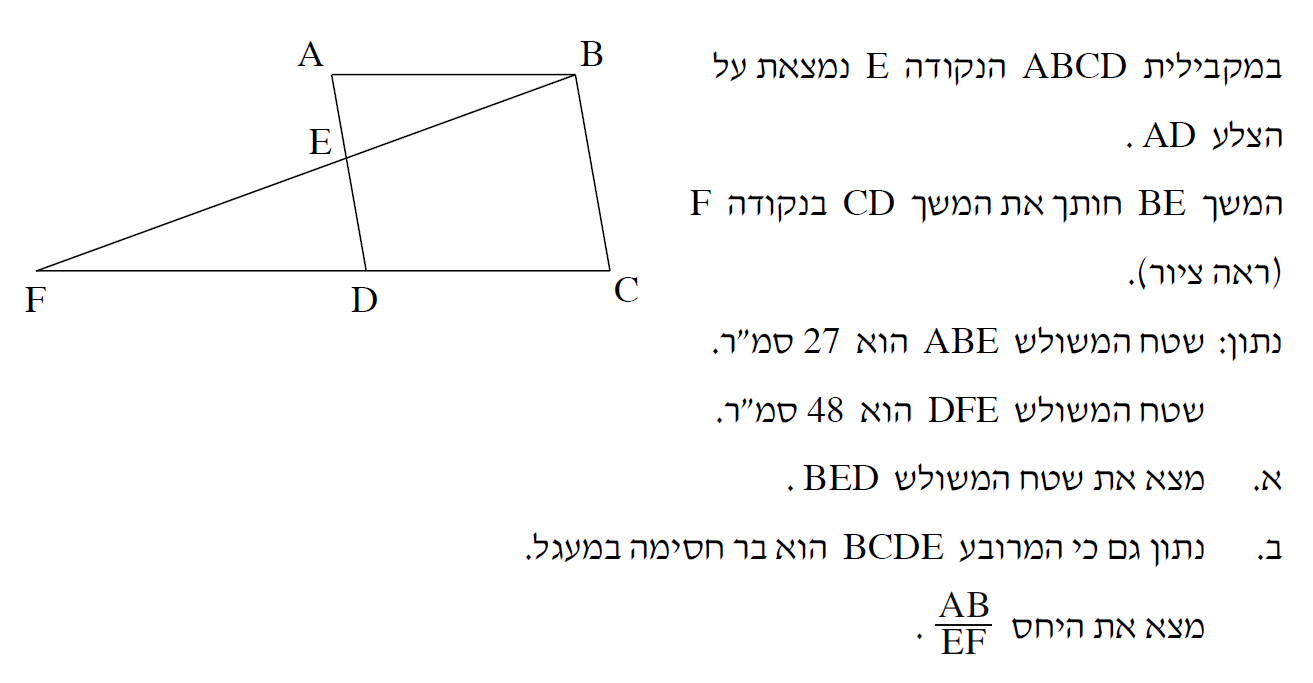
\includegraphics[width=\textwidth]{winter-2015-4}
\end{center}

\vspace{-5mm}

\textbf{סעיף א}

יש שתי דרכים לחשב את השטח של 
$\triangle BED$.
הראשונה היא לחשב את השטח של
$\triangle ABD$
ולהחסיר את השטח של
$\triangle ABE$.
לפי הסימונים בתרשים:
\[
S_{ABD}=\frac{1}{2}x(h_1+h_2)\,,\quad\quad S_{AEB}=\frac{1}{2}xh_1\,.
\]
אם נוכל לבטא את
$h_2$
במונחים של
$h_1$,
נוכל להחשב את
$S_{BED}=S_{ABD}-S_{AEB}$.

$\triangle ABE\sim \triangle DFE$
לפי ז.ז. בגלל הזוויות המתחלפות ב-%
$A,D$
ו-%
$B,F$.
לפי משפט
$100$%
ז "יחס השטחים שווה לריבוע יחס הדמיון":
\erh{12pt}
\begin{equationarray*}{rcl}
\frac{h_2}{h_1} &=& \sqrt{\frac{S_{DEF}}{S_{ABE}}} = \sqrt{\frac{48}{27}} = \frac{4}{3}\\
S_{BED} &=& S_{ABD}-S_{AEB}\\
&=& \frac{1}{2}x\left(h_1+\frac{4}{3}h_1\right)-\frac{1}{2}xh_1\\
%&=& \frac{1}{2}x\cdot \frac{4}{3}h_1\\
&=& \frac{4}{3}\left(\frac{1}{2}xh_1\right)=\frac{4}{3}\left(S_{ABE}\right)= \frac{4}{3}\cdot 27 = 36\,.
\end{equationarray*}

\vspace{-2mm}

\begin{center}
\selectlanguage{english}
\begin{tikzpicture}
\coordinate [label=below right:$D$] (D)  at (0,0);
\coordinate [label=below:$C$] (C)  at (4,0);
\coordinate [label=above right:$B$] (B)  at (3,3);
\coordinate [label=above left:$A$] (A)  at (-1,3);
\draw[thick,name path=para] (A) -- (B) -- (C) -- (D) -- cycle;
\node at (2,-.3) {$x$};
\node at (1.2,3.3) {$x$};
\path[name path=bf] (B) -- (-4,-.3);
\path[name path=df] (D) -- (-4,0);
\path[name intersections={of=bf and para,by={dummy,E}}];
\node[above left,xshift=-4pt] at (E) {$E$};
\path[name intersections={of=df and bf,by={F}}];
\node[below left] at (F) {$F$};
\draw[thick] (D) -- (F) -- (B);
\fill (A) circle (1.5pt);
\fill (B) circle (1.5pt);
\fill (C) circle (1.5pt);
\fill (D) circle (1.5pt);
\fill (E) circle (1.5pt);
\fill (F) circle (1.5pt);
\draw[thick,dashed] (E) |- (A);
\draw[thick,dashed] (E) |- (D);
\draw[thick,dashed] (B) -- (D);
\node at (-.1,2.4) {$h_1$};
\node at (-.8,.6) {$h_2$};
\end{tikzpicture}
\end{center}

\np

הדרך השנייה לחשב את השטח של
$\triangle BED$
קשה לראות אבל החישוב מאוד פשוט. למשולשים 
$\triangle AEB,\triangle BED$
גובה זהה 
$h$
מהנקודה
$B$
ועד
$AD$.
יחס השטחים הוא הריבוע של יחס הצלעות
$AE,ED$
במשולשים 
$\triangle ABE,\triangle DFE$
שחישבנו לעיל:
\[
S_{BED} = \frac{4}{3}S_{AEB}=\frac{4}{3}\cdot 27 = 36\,.
\]
\vspace{-2ex}

\begin{center}
\selectlanguage{english}
\begin{tikzpicture}
\coordinate [label=below:$D$] (D)  at (0,0);
\coordinate (C)  at (4,0);
\coordinate [label=above right:$B$] (B)  at (3,3);
\coordinate [label=above left:$A$] (A)  at (-1,3);
\path[thick,name path=para] (A) -- (B) -- (C) -- (D) -- cycle;
\path[name path=bf] (B) -- (-4,-.3);
\path[name path=df] (D) -- (-4,0);
\path[name intersections={of=bf and para,by={dummy,E}}];
\node[left,xshift=-4pt] at (E) {$E$};
\draw[thick] (A) -- (B) -- (E) -- cycle;
\draw[thick] (E) -- (D) -- (B);
\fill (A) circle (1.5pt);
\fill (B) circle (1.5pt);
\fill (D) circle (1.5pt);
\fill (E) circle (1.5pt);
\coordinate (H) at ($(A)!(B)!(D)$);
\draw[thick,dashed] (B) -- node[above left] {$h$} (H);
\fill (H) circle (1.5pt);
\draw[rotate=20] (H) rectangle +(7pt,7pt);
\end{tikzpicture}
\end{center}

\vspace{-2ex}

\textbf{סעיף ב}

לכאורה, לא צריך את הנתון על המרובע כי
$\triangle ABE\sim \triangle DFE$.
אבל עיון מדוקדק יגלה שהיחס שחישבנו הוא 
$\frac{AB}{FD}$
ולא
$\frac{AB}{EF}$.

הנתון שהמרובע 
$BCDE$
בר חסימה במעגל מכוון למשפט
$56$
"ניתן לחסום מרובע במעגל אם ורק אם סכום זוג זוויות נגדיות שווה ל-%
$180^\circ$".
נסמן זוויות ונראה אם יוצא מזה משהו מועיל. נסמן ב-%
$\alpha$
את הזוויות הנגדיות של המקבילית
$A,C$
ואת הזוויות המתאימות בנקודות
$C,D$.
נסמן ב-%
$\beta$
את הזוויות המתחלפות ב-%
$B,F$.

סכום הזוויות במשולש הוא
$180$
ולכן הזוויות הקודקודיות ב-%
$E$
שוות ל-%
$180-(\alpha+\beta)$.
לפי זוויות משלימות
$\angle BED=\alpha+\beta$.
נפעיל את משפט
$56$
ונקבל:
\erh{2pt}
\begin{equationarray*}{rcl}
\angle BCD + \angle BED&=&180\\
\alpha+\alpha+\beta&=&180\\
\alpha&=&180-(\alpha+\beta)\\
\angle ABE&=&\angle EBA\\
\angle 	DFE&=&\angle EFD\,. 
\end{equationarray*}
המשולשים
$\triangle ABE, \triangle DFE$ 
שווה שוקיים! נשתמש ביחס שחישבנו בסעיף א:
\[
\frac{AB}{EF} = \frac{AB}{FD} = \frac{3}{4}\,.
\]


\begin{center}
\selectlanguage{english}
\begin{tikzpicture}[scale=1.1]
\coordinate [label=below right:$D$] (D)  at (0,0);
\coordinate [label=below:$C$] (C)  at (4,0);
\coordinate [label=above right:$B$] (B)  at (3,3);
\coordinate [label=above left:$A$] (A)  at (-1,3);
\draw[thick,name path=para] (A) -- (B) -- (C) -- (D) -- cycle;
\path[name path=bf] (B) -- (-4,-.3);
\path[name path=df] (D) -- (-4,0);
\path[name intersections={of=bf and para,by={dummy,E}}];
\node[above left,xshift=-4pt,yshift=2pt] at (E) {$E$};
\path[name intersections={of=df and bf,by={F}}];
\draw[thick] (D) -- (F) -- (B);
\fill (A) node[below right,xshift=2pt] {$\alpha$} circle (1.5pt);
\fill (B) node[below left,xshift=-22pt,yshift=1pt] {$\beta$} circle (1.5pt);
\fill (C) node[above left,xshift=-2pt] {$\alpha$} circle (1.5pt);
\fill (D) node[above left,xshift=-2pt] {$\alpha$} circle (1.5pt);
\fill (E) node[right,xshift=3pt,yshift=-5pt] {$\alpha+\beta$} circle (1.5pt);
\fill (F) node[below left] {$F$} node[above right,xshift=28pt,yshift=-2pt] {$\beta$} circle (1.5pt);
\node at ($(E)+(-55pt,0)$) {$180-(\alpha+\beta)$};
\draw[->] ($(E)+(-20pt,2pt)$) -- +(24pt,3pt);
\draw[->] ($(E)+(-20pt,-2pt)$) -- +(19pt,-3pt);
\end{tikzpicture}
\end{center}


%%%%%%%%%%%%%%%%%%%%%%%%%%%%%%%%%%%%%%%%%%%%%%%%%%%%%%%%%%%%%%%%%%%


\np

\section{קיץ תשע"ד מועד ב}

\begin{center}
\selectlanguage{english}
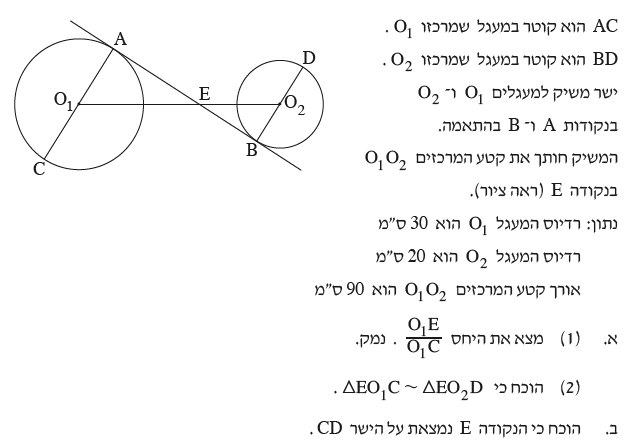
\includegraphics[width=.9\textwidth]{summer-2014b-4}
\end{center}

\vspace{-2ex}

\textbf{סעיף א}
$(1)$

כדי לסבך מעט את השאלה ביקשו את היחס בין
$O_1E$
ל-%
$O_1C$,
אבל 
$O_1A=O_1C$
כי הם רדיוסים. אם נוכיח ש-%
$\triangle O_1 A E\sim \triangle O_2 B E$,
נוכל להחשב את היחס המבוקש.

$AB$
משיק לשני המעגלים ולכן 
$\angle O_1 A E= \angle O_2 B E=90^\circ$
לפי משפט
$77$
"המשיק למעגל מאונך לרדיוס בנקודת ההשקה".
$\angle A E O_1=\angle B E O_2$
כי הן זוויות קודקודיות. מכאן ש-%
$\triangle O_1 A E\sim \triangle O_2 B E$
לפי ז.ז. נסמן ב-%
$x$
את אורכו של
$O_1 E$
ונקבל:
\erh{14pt}
\[
\begin{array}{l}
\displaystyle\frac{O_1 E}{O_2 E}= \frac{x}{90-x} = \frac{O_1A}{O_2B} = \frac{30}{20}\\
%2700-30x&=&20x\\
%x=54\\
\displaystyle\frac{O_1 E}{O_1 C} =\frac{O_1E}{O_1A} = \frac{54}{30}=\frac{9}{5}\,.
\end{array}
\]
\vspace{-2ex}

\begin{center}
\selectlanguage{english}
\begin{tikzpicture}[scale=1.1]
\coordinate (o1) at (0,0);
\coordinate (A)  at (50:2);
\draw[rotate=-130] (A) rectangle +(4pt,4pt);
\coordinate (C) at (-130:2);
\node [draw,circle through=(C)] at (o1) {};
\draw (A) -- (C);
\coordinate (o2) at (5,0);
\coordinate (D)  at ($(o2) + (50:1)$);
\coordinate (B)  at ($(o2) + (-130:1)$);
\draw[rotate=50] (B) rectangle +(4pt,4pt);
\node [draw,circle through=(B)] at (o2) {};
\draw (B) -- (D);
\draw[name path=diameters] (o1) -- node[below,xshift=4mm] {$90$} (o2);
\draw[name path=tangents] ($ (A) ! -.3 ! (B) $) -- ($ (A) ! 1.3 ! (B) $);
\path [name intersections={of=diameters and tangents,by={E}}];
\fill (A) node[above,xshift=2pt] {$A$} circle(1pt);
\fill (B) node[below,xshift=-4pt] {$B$} circle(1pt);
\fill (C) node[below,xshift=-2pt] {$C$} circle(1pt);
\fill (D) node[above,xshift=4pt] {$D$} circle(1pt);
\fill (E) node[above,xshift=2pt] {$E$} circle(1pt);
\fill (o1) node[left,xshift=-2pt] {$O_1$} circle(1pt);
\fill (o2) node[right,xshift=2pt] {$O_2$} circle(1pt);
\path (A)  -- node[left,xshift=-2pt] {$30$} (o1);
\path (o1) -- node[left,xshift=-2pt] {$30$} (C);
\path (D)  -- node[right,xshift=1pt] {$20$} (o2);
\path (o2) -- node[right,xshift=1pt] {$20$} (B);
\path (o1) -- node[above] {$x$} (E);
\end{tikzpicture}
\end{center}

\np

\textbf{סעיף א
$(2)$}

נראה שאפשר להשתמש באותה שיטה כדי להוכיח שהמשולשים 
$\triangle E O_1 C \sim \triangle E O_2 D$
דומים. אבל, כפי שמרמז סעיף ב, איננו יודעים שהנקודה
$E$
נמצאת על הקו הישר
$CD$,
ולכן איננו יכולים להניח ש-%
$\angle O_1 E C, \angle O_2 E D$
הן זוויות הקודקודיות )שוות(. במקום זה, נשתמש בעובדה שהקוטרים מקביליים ולהוכיח בצורה ישירה שהמשולשים דומים.

$AC\|DB$
כי שניהם ניצבים לקו
$O_1O_2$,
ולכן 
$\angle C O_1 E=\angle D O_2 E=\alpha$
כי הן זוויות מתחלפות. כל הרדיוסים של מעגל שווים, כך ש-%
$O_1C=O_1A, O_2B=O_2D$.
הוכחנו ש-%
$\triangle E O_1 A \sim \triangle E O_2 B$,
ולכן
\[
\frac{O_1E}{O_2E}=\frac{O_1C}{O_2D}\,,
\]
ו-%
$\triangle E O_1 C \sim \triangle E O_2 D$.

\vspace{-1ex}

\begin{center}
\selectlanguage{english}
\begin{tikzpicture}[scale=1.1]
\coordinate (o1) at (0,0);
\coordinate (A)  at (50:2);
\draw[rotate=-130] (A) rectangle +(4pt,4pt);
\coordinate (C) at (-130:2);
\node [draw,circle through=(C)] at (o1) {};
\draw (A) -- (o1);
\draw[dashed,very thick] (o1) -- (C);
\coordinate (o2) at (5,0);
\coordinate (D)  at ($(o2) + (50:1)$);
\coordinate (B)  at ($(o2) + (-130:1)$);
\node[below right] at (o1) {$\alpha$};
\node[above left,xshift=1mm] at (o2) {$\alpha$};
\draw[rotate=50] (B) rectangle +(4pt,4pt);
\node [draw,circle through=(B)] at (o2) {};
\draw (B) -- (o2);
\draw[dashed,very thick] (o2) -- (D);
\draw[name path=diameters,dashed,very thick] (o1) -- node[below,xshift=6mm,yshift=-2mm] {$90$} (o2);
\draw[name path=tangents] ($ (A) ! -.3 ! (B) $) -- ($ (A) ! 1.3 ! (B) $);
\path [name intersections={of=diameters and tangents,by={E}}];
\path[dashed,very thick] (o1) -- node[above] {$x$} (E);
\draw[dashed,very thick] (C) -- (D);
\fill (A) node[above,xshift=2pt] {$A$} circle(1pt);
\fill (B) node[below,xshift=-4pt] {$B$} circle(1pt);
\fill (C) node[below,xshift=-2pt] {$C$} circle(1pt);
\fill (D) node[above,xshift=4pt] {$D$} circle(1pt);
\fill (E) node[above,xshift=2pt] {$E$} circle(1pt);
\fill (o1) node[left,xshift=-2pt] {$O_1$} circle(1pt);
\fill (o2) node[right,xshift=2pt] {$O_2$} circle(1pt);
\path (A)  -- node[left,xshift=-2pt] {$30$} (o1);
\path (o1) -- node[left,xshift=-2pt] {$30$} (C);
\path (D)  -- node[right,xshift=1pt] {$20$} (o2);
\path (o2) -- node[right,xshift=1pt] {$20$} (B);
\path (o1) -- node[above] {$x$} (E);
\end{tikzpicture}
\end{center}

\vspace{-1ex}

\textbf{סעיף ב}

נתבונן בזוויות סביב הנקודה
$E$
שנמצאת על 
$CD$
אם הזווית 
$\angle AED$
משלימה לזווית
$\angle AEC$.
הוכחנו
$\triangle O_1 E C\sim \triangle O_2 E D$
ו-%
$\triangle O_1 A E \sim \triangle O_2 B E$,
ונסמן את הזוויות השוות
$\alpha,\beta$.
נתון ש-%
$AB$
הוא קו ישר ו-% 
$\angle AED$
משלימה ל-%
$\angle DEB$,
כך ש-%
$\angle AED = 180^\circ - (\alpha + \beta)$.
נבדוק עם 
$\angle AED$
משלימה ל-%
$\angle AEC$:
\[
\angle AED + \angle AEC = (180^\circ - (\alpha + \beta)) + (\alpha + \beta) = 180^\circ\,.
\]

\vspace{-3ex}

\begin{center}
\selectlanguage{english}
\begin{tikzpicture}[scale=1.1]
\coordinate [label=left:$O_1$] (o1) at (0,0);
\coordinate [label=above:$A$] (A)  at (50:2);
\coordinate [label=below:$C$] (C) at (-130:2);
\node [circle through=(C)] at (o1) {};
\draw (A) -- (C);
\coordinate [label=right:$O_2$] (o2) at (5,0);
\coordinate [label=above:$D$] (D)  at ($(o2) + (50:1)$);
\coordinate [label=below:$B$] (B)  at ($(o2) + (-130:1)$);
\node [circle through=(B)] at (o2) {};
\draw (B) -- (D);
\draw[name path=diameters] (o1) -- (o2);
\draw[name path=tangents] ($ (A) ! -.1 ! (B) $) -- ($ (A) ! 1.1 ! (B) $);
\path [name intersections={of=diameters and tangents,by={[label=above:$E$]E}}];
\path (A)  -- (o1);
\path (o1) -- (C);
\path (D)  -- (o2);
\path (o2) -- (B);
\path (o1) -- (E);
\node[xshift=-20pt,yshift=7pt] at (E) {$\alpha$};
\node[xshift=20pt,yshift=-7pt] at (E) {$\alpha$};
\node[xshift=38pt,yshift=6pt] at (E) {$\beta$};
\node[xshift=-38pt,yshift=-7pt] at (E) {$\beta$};
\draw (C) -- (D);
\end{tikzpicture}
\end{center}
%%%%%%%%%%%%%%%%%%%%%%%%%%%%%%%%%%%%%%%%%%%%%%%%%%%%%%%%%%%%%%%%%%%


\np
\section{קיץ תשע"ד מועד א}

\begin{center}
\selectlanguage{english}
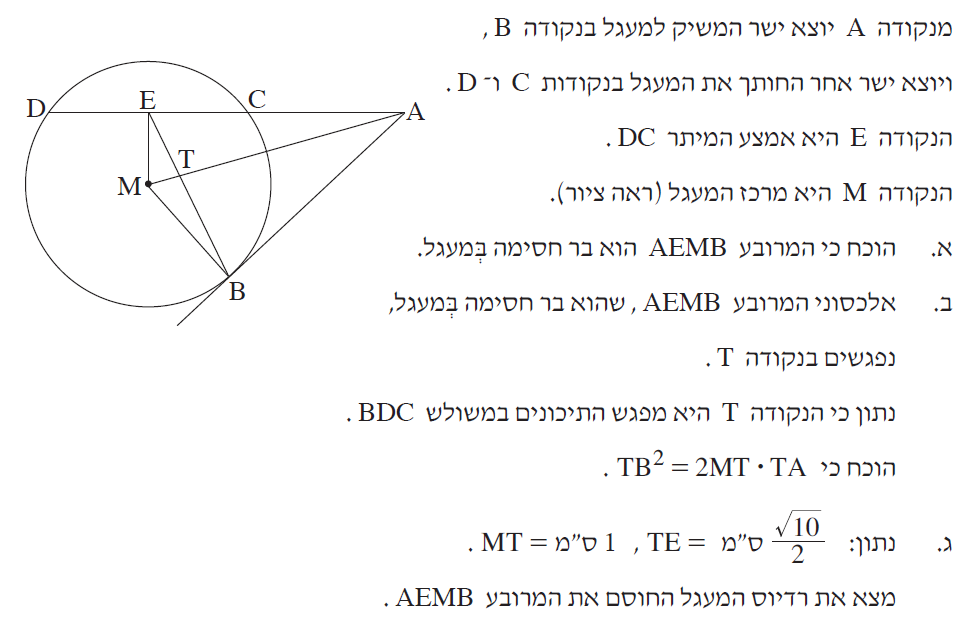
\includegraphics[width=\textwidth]{summer-2014a-4}
\end{center}

\vspace{-2ex}

\textbf{סעיף א}

משפטים רלוונטיים: 
$(103)$
"אם מנקודה שמחוץ למעגל יוצאים חותך ומשיק, אז מכפלת החותך בחלקו החיצוני שווה לריבוע המשיק",
$AB^2=AC\cdot AD$.
$(77)$
"המשיק למעגל מאונך לרדיוס בנקודת ההשקה",
$MB \perp AB$. 
$(68)$
"קטע ממרכז המעגל החוצה את המיתר מאונך למיתר",
$ME\perp DC$.
$(56)$
"ניתן לחסום מרובע במעגל רק אם סכום הזוויות הנגדיות שווה ל-%
$180^\circ$",
ב-%
$AEMB$:
\[
\angle MEA+\angle MBA=\angle EMB+\angle EAB=180^\circ\,.
\]
מ-%
$MB \perp AB$
ו-%
$ME\perp DC$,
$\angle MEA + \angle MBA = 180^\circ$.
לפי משפט
$(106)$
"סכום הזוויות הפנימיות של מצולע קמור הוא
$180^\circ(n-2)$",
סכום הזוויות הפנימיות של מרובע הוא 
$360^\circ$,
ולכן:
\[
\angle EMB + \angle EAB = 360^\circ -(\angle MEA + \angle MBA) = 180^\circ\,.
\]
\vspace{-4ex}
\begin{center}
\selectlanguage{english}
\begin{tikzpicture}[scale=.8]
\coordinate [label=left:$M$] (M) at (0,0);
\coordinate [label=below right:$B$] (B)  at (-45:3);
\coordinate [label=right:$A$] (A) at (6,2);
\node [draw,thick,circle through=(B),name path=circ] at (M) {};
\draw[name path=tangents,thick] (A) -- ($ (A) ! 1.3 ! (B) $);
\path[name path=adc] (A) -- +(-9,0);
\path[name intersections={of=adc and circ,by={[label=above right:$C$]C,[label=above left:$D$]D}}];
\draw[thick] (A) -- (D);
\draw[thick,name path=am] (A) -- (M);
\draw[thick] (B) -- (M);
\path[name path=mid] (M) -- +(0,3.5);
\path[name intersections={of=mid and adc,by={[label=above:$E$]E}}];
\draw[thick,name path=eb] (E) -- (B);
\draw[thick] (E) -- (M);
\path[name intersections={of=eb and am,by={T}}];
\fill (T) node[above,xshift=4pt] {$T$} circle(1.5pt);
\fill (M) circle (1.5pt);
\fill (A) circle (1.5pt);
\fill (B) circle (1.5pt);
\fill (C) circle (1.5pt);
\fill (D) circle (1.5pt);
\fill (E) circle (1.5pt);
\draw[rotate=180] (E) rectangle +(7pt,7pt);
\draw[rotate=140] (B) rectangle +(7pt,7pt);
\end{tikzpicture}
\end{center}

\np

\textbf{סעיף ב}

באיור למטה מופיע המידע הרלוונטי בלבד: המעגל החוסם את המרובע
$AEMB$,
האלכסונים שלו
$AM,EB$
והמשולש
$BDC$.
$AM,EB$
הם מיתרים נחתכים של המעגל החוסם. לפי משפט
$(101)$
"אם במעגל שני מיתרים נחתכים, אז מכפלת קטעי מיתר אחד שווה למכפלת קטעי המיתר השני",
$TB\cdot TE=MT\cdot TA$.
אם נוכיח
$TE=TB/2$,
נקבל הוכחה להמשוואה בשאלה.
נתון שהנקודה
$T$
היא מפגש התיכונים ב-%
$\triangle BDC$
ולפי משפט
$(46)$
"נקודת חיתוך התיכונים מחלקת כל תיכון ביחס
$2:1$",
כאן
$TB/TE=2/1$
או
$TE=TB/2$.

\vspace{-10ex}
\begin{center}
\selectlanguage{english}
\begin{tikzpicture}[scale=.8]
\coordinate [label=left:$M$] (M) at (0,0);
\coordinate [label=below right:$B$] (B)  at (-45:3);
\coordinate [label=right:$A$] (A) at (6,2);
\node [circle through=(B),name path=circ] at (M) {};
\draw[name path=tangents,thick] (A) -- (B);
\path[name path=adc] (A) -- +(-9,0);
\path[name intersections={of=adc and circ,by={[label=above right:$C$]C,[label=above left:$D$]D}}];
\draw[thick,name path=am] (A) -- (M);
\draw[thick] (B) -- (M);
\path[name path=mid] (M) -- +(0,3.5);
\path[name intersections={of=mid and adc,by={[label=above left:$E$]E}}];
\draw[thick,name path=eb] (E) -- (B);
\path[name intersections={of=eb and am,by={T}}];
\fill (T) node[above,xshift=4pt] {$T$} circle(1.5pt);
\draw[thick] (E) -- (M);
\path (E) -- node[right] {$a$} (T) -- node[above,xshift=4pt,yshift=4pt] {$2a$} (B);
\fill (M) circle (1.5pt);
\fill (A) circle (1.5pt);
\fill (B) circle (1.5pt);
\fill (C) circle (1.5pt);
\fill (D) circle (1.5pt);
\fill (E) circle (1.5pt);
\draw[very thick,dashed] (C) -- (B) -- (D) -- cycle;
\tkzCircumCenter(M,E,A)\tkzGetPoint{O}
\tkzDrawCircle[thick](O,A)
\draw[rotate=180] (E) rectangle +(7pt,7pt);
\draw[rotate=50] (B) rectangle +(7pt,7pt);
\end{tikzpicture}
\end{center}
\vspace{-10ex}

\textbf{סעיף ג}

רדיוס המעגל החוסם הוא קו מהמרכז לאחת הקוקודים
$A,E,M,B$.
אין אנו יודעים את מרכז המעגל, אבל נראה ש-%
$MA$
יכול להיות קוטר ואז נקבל את הרדיוס כמחצית הקוטר.

מסעיף א
$\angle MBA$
היא זווית ישרה, ולפי משפט
$(74)$
"זווית היקפית בת
$90^\circ$
נשענת על קוטר",
$MA$
הוא קוטר. עם הערכים הנתונים נחשב את הרדיוס תוך שימוש בנוסחאות מסעיף ב:
\erh{16pt}
\begin{equationarray*}{rcl}
R &=& \frac{1}{2}MA\\
&=&\frac{1}{2}(MT+TA)\\
&=&\frac{1}{2}\left(MT+\frac{TB^2}{2MT}\right)\\
&=&\frac{1}{2}\left(MT+\frac{4TE}{2MT}\right)\\
&=&\frac{1}{2}\left(1+\frac{1}{2\cdot 1}\cdot 4\left(\frac{\sqrt{10}}{2}\right)^2\right)\\
&=&3\,.
\end{equationarray*}

%%%%%%%%%%%%%%%%%%%%%%%%%%%%%%%%%%%%%%%%%%%%%%%%%%%%%%%%%%%%%%%%%%%



\np

\section{חורף תשע"ד}

\begin{center}
\selectlanguage{english}
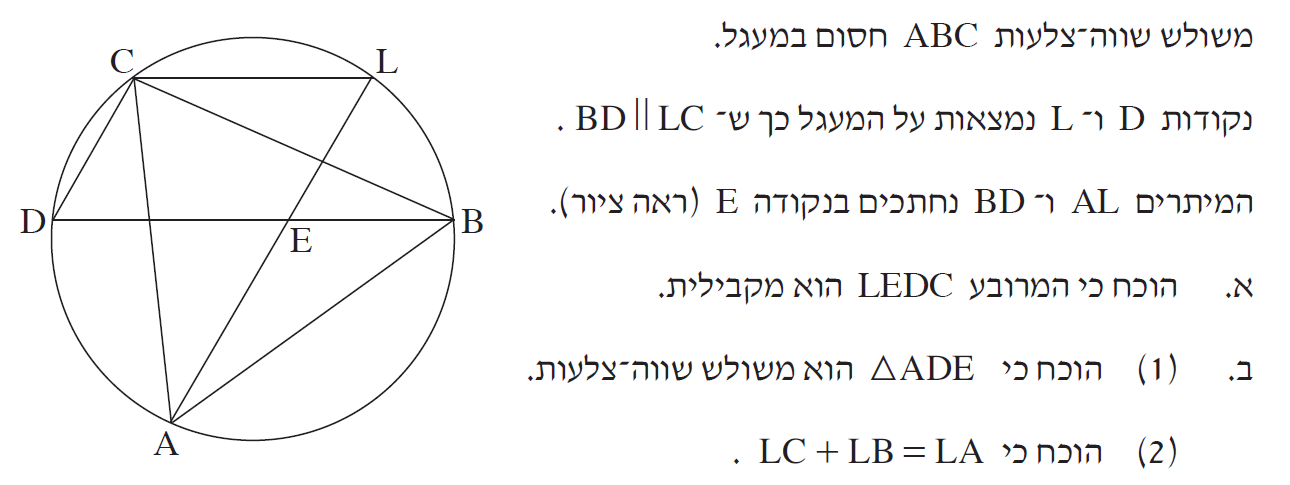
\includegraphics[width=\textwidth]{winter-2014-4}
\end{center}

\vspace{-2ex}

\textbf{סעיף א}

אין לנו מידע על המיתרים המגדירים את המרובע, לכן ננסה להוכיח שהוא מקבילית לפי משפט
$29$
"מרובע שבו כל זוג זוויות נגדיות שוות הוא מקבילית". כאשר יש "מספר רב" של מיתרים, סביר שיש זוויות שוות לפי משפט
$72$
"במעגל, כל הזוויות ההיקפיות הנשענות על מיתר מאותו צד של המיתר שוות זו לזו". נסמן את הזוויות של המשולש שווה צלעות
$\triangle ABC$
ב-%
$\alpha=60^\circ$.


$\angle CLA=\angle CBA=\alpha$
כי הן נשענות על המיתר
$AC$.
$\angle CDB=\angle CAB=\alpha$
כי הן נשענות על המיתר
$BC$.
נתון ש-%
$BD\|LC$,
אז
$\angle LEB = \angle CLA = \alpha$
לפי זוויות מתחלפות.

מה עם זוג הזוויות הנגדיות השני במרובע? 
$\angle LED=180-\alpha$
לפי זוויות משלימות בנקודה
$E$.
נתון ש-%
$BD\|LC$
ולכן
$\angle LCD=180-\angle DCB=180-\alpha$
לפי זוויות חד-צדדיות על 
$CD$.
\vspace{-2ex}
\begin{center}
\selectlanguage{english}
\begin{tikzpicture}[scale=.95]
\coordinate (left) at (0,0);
\coordinate (right) at (6,0);
\coordinate (apath) at (0,-4);
\coordinate (bpath) at (7,1);
\coordinate (cpath) at (1.5,4);
\path [name path=chord1] (apath) -- (bpath);
\path [name path=chord2] (apath) -- (cpath);
\coordinate (center) at ($ (right)!.5!(left) $);
\node [draw,thick,circle through=(left),name path=circ] at (center) {};
\path [name intersections={of=circ and chord1,by={b,a}}];
\path [name intersections={of=circ and chord2,by={c,dummy1}}];
\fill (a) circle (2pt) node[below left] {$A$} node[xshift=4pt,yshift=15pt] {$\alpha$};
\fill (b) circle (2pt) node[right] {$B$} node[xshift=-15pt,yshift=-5pt] {$\alpha$};
\fill (c) circle (2pt) node[above left] {$C$} node[xshift=6pt,yshift=-10pt] {$\alpha$};
\path [name path=chord3] (b) -- +(-7,0);
\path [name intersections={of=circ and chord3,by={d}}];
\fill (d) circle (2pt) node[left] {$D$} node[above right,xshift=4pt,yshift=-2pt] {$\alpha?$};
\path [name path=chord4] (c) -- +(4,0);
\path [name intersections={of=circ and chord4,by={l}}];
\fill (l) circle (2pt) node[above right] {$L$} node[below left,xshift=-4pt] {$\alpha?$};
%% Draw triangle
\draw[thick,name path=chord5] (l) -- (a);
\draw [name intersections={of=chord5 and chord3,by={e}}];
\fill (e) circle (2pt) node[below right] {$E$} node[above right,xshift=4pt,yshift=-2pt] {$\alpha?$};
\draw[thick] (a) -- (b) -- (c) -- cycle;
\draw[thick] (b) -- (e);
\draw[very thick] (e) -- (d) -- (c) -- (l) -- cycle;
%% Angles
\draw[thick] +($ (a)!.15!(b) $) arc [radius=18pt,start angle=20,delta angle=82];
\draw[thick] ($ (c)!.15!(b) $) arc [radius=18pt,start angle=-20,delta angle=-75];
\draw[thick] ($ (b)!.15!(c) $) arc [radius=18pt,start angle=140,delta angle=82];
\end{tikzpicture}
\end{center}

\np

\textbf{סעיף ב}
$(1)$

שוב אין לנו מידע על אורכי הצלעות, לכן ננסה להוכיח שכל הזוויות של המשולש
$\triangle ADE$
שוות. מספיק להוכיח ששתי זוויות שוות ל-%
$60^\circ$
כי השלישית צריכה להשלים ל-%
$180^\circ$.

בסעיף א הוכחנו ש-%
$\angle LEB=\angle CLA=\angle CBA=60^\circ$.
מכאן ש-%
$\angle DEA=\angle LEB=60^\circ$
לפי זוויות קודקודיות. כי הן זוויות קודקודיות. ננסה להוכיח ש-%
$\angle DAE=\angle DAL=60^\circ$
או
$\angle ADE=\angle ADB=60^\circ$
על ידי חיפוש זוויות הנשענת על המיתר
$DL$
או
$AB$.
אכן,
$\angle ADB=$
ו-%
$\angle ACB=60^\circ$
נשענות על המיתר
$AB$.

\vspace{-4ex}
\begin{center}
\selectlanguage{english}
\begin{tikzpicture}[scale=.95]
\coordinate (left) at (0,0);
\coordinate (right) at (6,0);
\coordinate (apath) at (0,-4);
\coordinate (bpath) at (7,1);
\coordinate (cpath) at (1.5,4);
\path [name path=chord1] (apath) -- (bpath);
\path [name path=chord2] (apath) -- (cpath);
\coordinate (center) at ($ (right)!.5!(left) $);
\node [draw,thick,circle through=(left),name path=circ] at (center) {};
\path [name intersections={of=circ and chord1,by={b,a}}];
\path [name intersections={of=circ and chord2,by={c,dummy1}}];
\fill (a) circle (2pt) node[below left] {$A$} node[xshift=9pt,yshift=40pt] {$60^\circ ?$};
\fill (b) circle (2pt) node[right] {$B$};
\fill (c) circle (2pt) node[above left] {$C$} node[xshift=16pt,yshift=-25pt] {$60^\circ$};
\path [name path=chord3] (b) -- +(-7,0);
\path [name intersections={of=circ and chord3,by={d}}];
\fill (d) circle (2pt) node[left] {$D$} node[below right,xshift=8pt] {$60^\circ ?$};
\path [name path=chord4] (c) -- +(4,0);
\path [name intersections={of=circ and chord4,by={l}}];
\fill (l) circle (2pt) node[above right] {$L$} ;
%% Draw triangle
\draw[thick,name path=chord5] (l) -- (a);
\path [name intersections={of=chord5 and chord3,by={e}}];
\draw[thick] (a) -- (c) -- (b) -- cycle;
\draw[thick] (b) -- (e);
\fill (e) circle (2pt) node[below right] {$E$} node[above right,xshift=4pt,yshift=-2pt] {$60^\circ$} node[below left,xshift=-4pt] {$60^\circ$};
%% Angles
\draw[thick] +($ (a)!.2!(e) $) arc [radius=12pt,start angle=20,delta angle=125];
\draw[thick] ($ (c)!.15!(b) $) arc [radius=18pt,start angle=-20,delta angle=-75];
\draw[very thick] (a) -- (d) -- (e) -- cycle;
\draw[thick] (c) -- (l) -- (b);
\draw[thick,dashed] (c) -- (d);
\end{tikzpicture}
\end{center}
\vspace{-4ex}

\textbf{סעיף ב
$(2)$}

מהחלק הראשון של הסעיף אנו יודעים ש-%
$\triangle ADE$
שווה צלעות,
$AE=DE$,
ו-%
$LC=DE$
כי הם צלעות נגדיים של המקבילית. לכן
$AE=LC$
ו:
\[
LA-LC=(LE+AE)-LC=(LE+LC)-LC=LE\,.
\]
נשאר להוכיח
$LE=LB$.
הוכחנו ש-%
$\angle LEB=60^\circ$,
כך שאם נוכיח שאחת מ-%
$\angle EBL,\angle ELB$
שווה ל-%
$60^\circ$
נקבל משלוש שווה צלעות. שוב נחפש זוויות הנשענות על אותו מיתר ונקבל ש-%
$\angle BLA=\angle BCA=60^\circ$
כי שתיהן נשענות על המיתר
$AB$.

תוך כי נסיונות לפתור את השאלה, מצאתי הוכחה אחרת מעניינת. 
$\angle LBD, \angle DCL$
נשענות על אותו קשת אבל
\textbf{מצדדים נגדיים}.
זווית היקפית שנשענת על קשת שווה למחצית הזווית המרכזית הנשענת על אותה קשת )משפט
$69$(,
ולכן אם סכום שתי הקשתות הוא כל המעגל, סכום הזוויות שווה 
$180^\circ$.
במקבילית,
$\angle DCL=120^\circ$,
ולכן:
\[
\angle LBE=\angle LBD=180^\circ - \angle DCL= 180^\circ - 120^\circ =60^\circ\,.
\]

%%%%%%%%%%%%%%%%%%%%%%%%%%%%%%%%%%%%%%%%%%%%%%%%%%%%%%%%%%%%%%%%%%%


\np

\section*{המלצות: גיאומטריה}

\addcontentsline{cot}{chapter}{המלצות: גיאומטריה}

\begin{itemize}
\item
חשוב לצייר תרשימים 
\textbf{ברורים וגדולים}
עדיף עם סרגל ומחוגה. בתהליך הפתרון אנו מסמנים את המידע המצטבר על הזוויות והצלעות ויש לדאוג שיהיה מספיק מקום.
\item
כאשר לשאלה יש מספר סעיפים כדאי לצייר תרשימים נפרדים לכל סעיף תוך העלמת מידע לא רלוונטי לאותו סעיף.

\item
\textbf{אין לסמוך על התרשים}.
לעתים, מה שנראה ברור בתרשים הוא בדיוק מה שעלינו להוכיח. בנספח א' הבאתי הוכחה שכל משולש הוא שווה שוקיים כאשר ההוכחה מסתמכת על תרשים שאינו נכון. מטרת התרשימים היא לחפש קשרים בין זוויות, צלעות, משיקים, וכו', כדי להעלות השערות על דרכים אפשרויות להוכחת הטענות.

\item
אני מעדיף לסמן זוויות עם אותיות יווניות כגון
$\alpha$,
ולא על ידי ציון שלושת הנקודות המגדירות אותה
$\angle ABC$.
הסיבה היא שקשה יותר לעקוב אחר הנקודות השונות של הזוויות מלעקוב אחר סימן בודד.

\item
רצוי לרשום את המשפטים שיכולים להיות רלוונטיים לפני שמנסים לפתור את השאלה כי זה יכול לכוון לפתרון. כמובן שלא כל המשפטים יהיו נחוצים. לעתים קרובות שאלה מתבססת על משפט מתקדם אחד, כגון הזוויות של מרובע החסום במעגל, הזווית בין משיק למעגל או השוויון של כל זווית היקפית הנשענת על מיתר. לכן, ההיכרות עם משפטים אלה יקל על מציאת פתרונות השאלות.

\item
יש משפטים שזוכרים בקלות כי הם די אינטואטיביים, למשל, שמשולשים חופפים לפי צ.צ.צ. ודומים לפי ז.ז. יש משפטים אחרים שקשה יותר לזכור אותם ושהוכחת נכונותם לא קלה. למשל, אני מתקשה לזכור איך להפעיל את המשפט על משיק ומיתר. בנספח ב' הבאתי תרשיםיים צבעוניים של מבחר משפטים בתקווה שהתרשימים יקלו עליכם לזכור אותם, בוודאי יחסית לניסוחים מילוליים מסורבלים.

\item
כאשר שואלים על שטחים של משולשים יש לחפש גבהים משותפים. אנו רגילים לראות גבהים שיורדים מנקודה לקו אופקי, אבל גבהים יכולים להופיע מכל נקודה לקו ממול ללא קשר למצג של המשולש על הנייר.

\item
כדי להוכיח חפיפה של משלושים ישר זווית, מספיק להוכיח שוויון של צלע אחד וזווית חדה אחת מכל משולש. אם הצלע הוא בין זווית חדה לבין הזווית הישרה, החפיפה היא מיידית לפי ז.צ.ז. אם הצלע הוא בין שתי הזוויות החדות )היתר(, זווית שערכה 
$\alpha$
ושנייה שערכה
$\beta$,
אזי
$\beta=90^\circ-\alpha$,
ושוב יש ז.צ.ז. אני מניח שבבחינה צריך לרשום איך מגיעים מזווית חדה וצלע לז.צ.ז., אבל כאשר מחפשים הוכחה לחפיפה קיצור דרך זה יכול להועיל.

\end{itemize}

